\chapter{Methods}
\label{Methods}
\section{Project Overview}
To help complete this Master thesis, I created various tools that would help create the final model outputs.
The project is divided into four parts. 
\begin{itemize}
    \item Using a GUI network creation too to define the number of phages, bacteria and resources in the network, and their interactions. 
    \item The simulation framework handles the data, runs the ODE simulations, and sends the data back to the dashboard. 
    \item A dashboard that the user can interact with to run simulations, edit parameter values, and plot and interact with the visualizations. 
    \item Download the data to create your own custom visualizations and analyses. 
\end{itemize}

A flowchart showing the user-system interactions can be seen in \Cref{AppendixC}. 

\subsection{Network Creation Tool}
\label{sec:network_creation_tool}
The user uses the GUI network creation tool to create and edit the network interactions. 
There are three types of variables in the simulations: phages, bacteria, and resources. 
Every node in the network represents either a phage, bacteria, or resource. 
The bacteria can be further divided into uninfected and infected bacteria. 
An edge links two nodes together if there is an arbitrary interaction occurring between them. 
Bacteria are infected by phages and take up resource. 
Which phage can infect which bacteria and which resources each species of bacteria can take up describes a network of interactions. 
Finally, the user can export (and later import to edit) the network representation for use in \Cref{sec:simulation_framework}, \Cref{sec:visualization_framework}, and \Cref{sec:custom_visualizations_and_framework}. 
\Cref{fig:ss:GUI_tool_and_network} shows the layout of the GUI tool and example networks that can be created. 

Every node represents a unique entity, and each entity has their own intrinsic properties. 
The user can intuitively define entities, their interactions, environmental and model settings using the GUI tool. 
This tool allows users to quickly and intuitively define entities and their attributes, entity interactions and their attributes, environmental data, and model settings.
An edge links two entities together if there is an arbitrary interaction occurring between the entities, with the properties exhibited in the interaction dependent on the interacting entities. 
Self interactions are allowed in the network. 
There is an environment node that is used to store global environmental data, such as the temperature and pH of the system.
The settings node holds information such as simulation length, max time step, and the type of ODE solver to use.
The tool provides functionalities for adding, editing, and visualizing nodes and edges, as well as importing and exporting the network structure.  

Once the user is happy with the graph shape, they can export the network representation for use in \Cref{sec:simulation_framework}, \Cref{sec:visualization_framework}, and \Cref{sec:custom_visualizations_and_framework}. 
The most important part is that the user defines the shape and the attributes of the network, as that can't be edited in part 2 onwards. 
It is possible go back to the network creation tool and upload the graph to the tool to be able to edit the network representation. \newline
The user can edit the values of the attributes in \Cref{sec:visualization_framework}, so the parameter values do not have to be perfect. 
As such, the user does not need to keep on using the GUI tool to edit parameter values. 

\Cref{fig:ss:initial_startup_GUI_tool} shows the layout of the GUI tool. \Cref{fig:ss:example_network} shows an example network that can be created.
There are numerous buttons that can be used to edit the graph, for example adding or removing nodes and edges. 
By default, an environment node holding parameters such as pH and temperature is added.
A settings node is added as well, holding settings data to be used for the solver, like the type of solver or simulation length.
Manually adding nodes and edges can get tedious and repetitive for large graphs, so the user can add multiple nodes and edges at the same time.
Nothing can interact with the environment and setting node, as they are used to hold data about the environment and network solver.
The user can alter the default attribute name and value by importing the GUI tool class and overriding the method implementation implementing the default names and values. 
The user can self-decide which parameter values to give, and if and how the parameter values are randomized. 

\begin{figure}
    \centering
    \begin{subfigure}{0.49\linewidth}
        \centering
        \captionsetup{width=1\linewidth}
        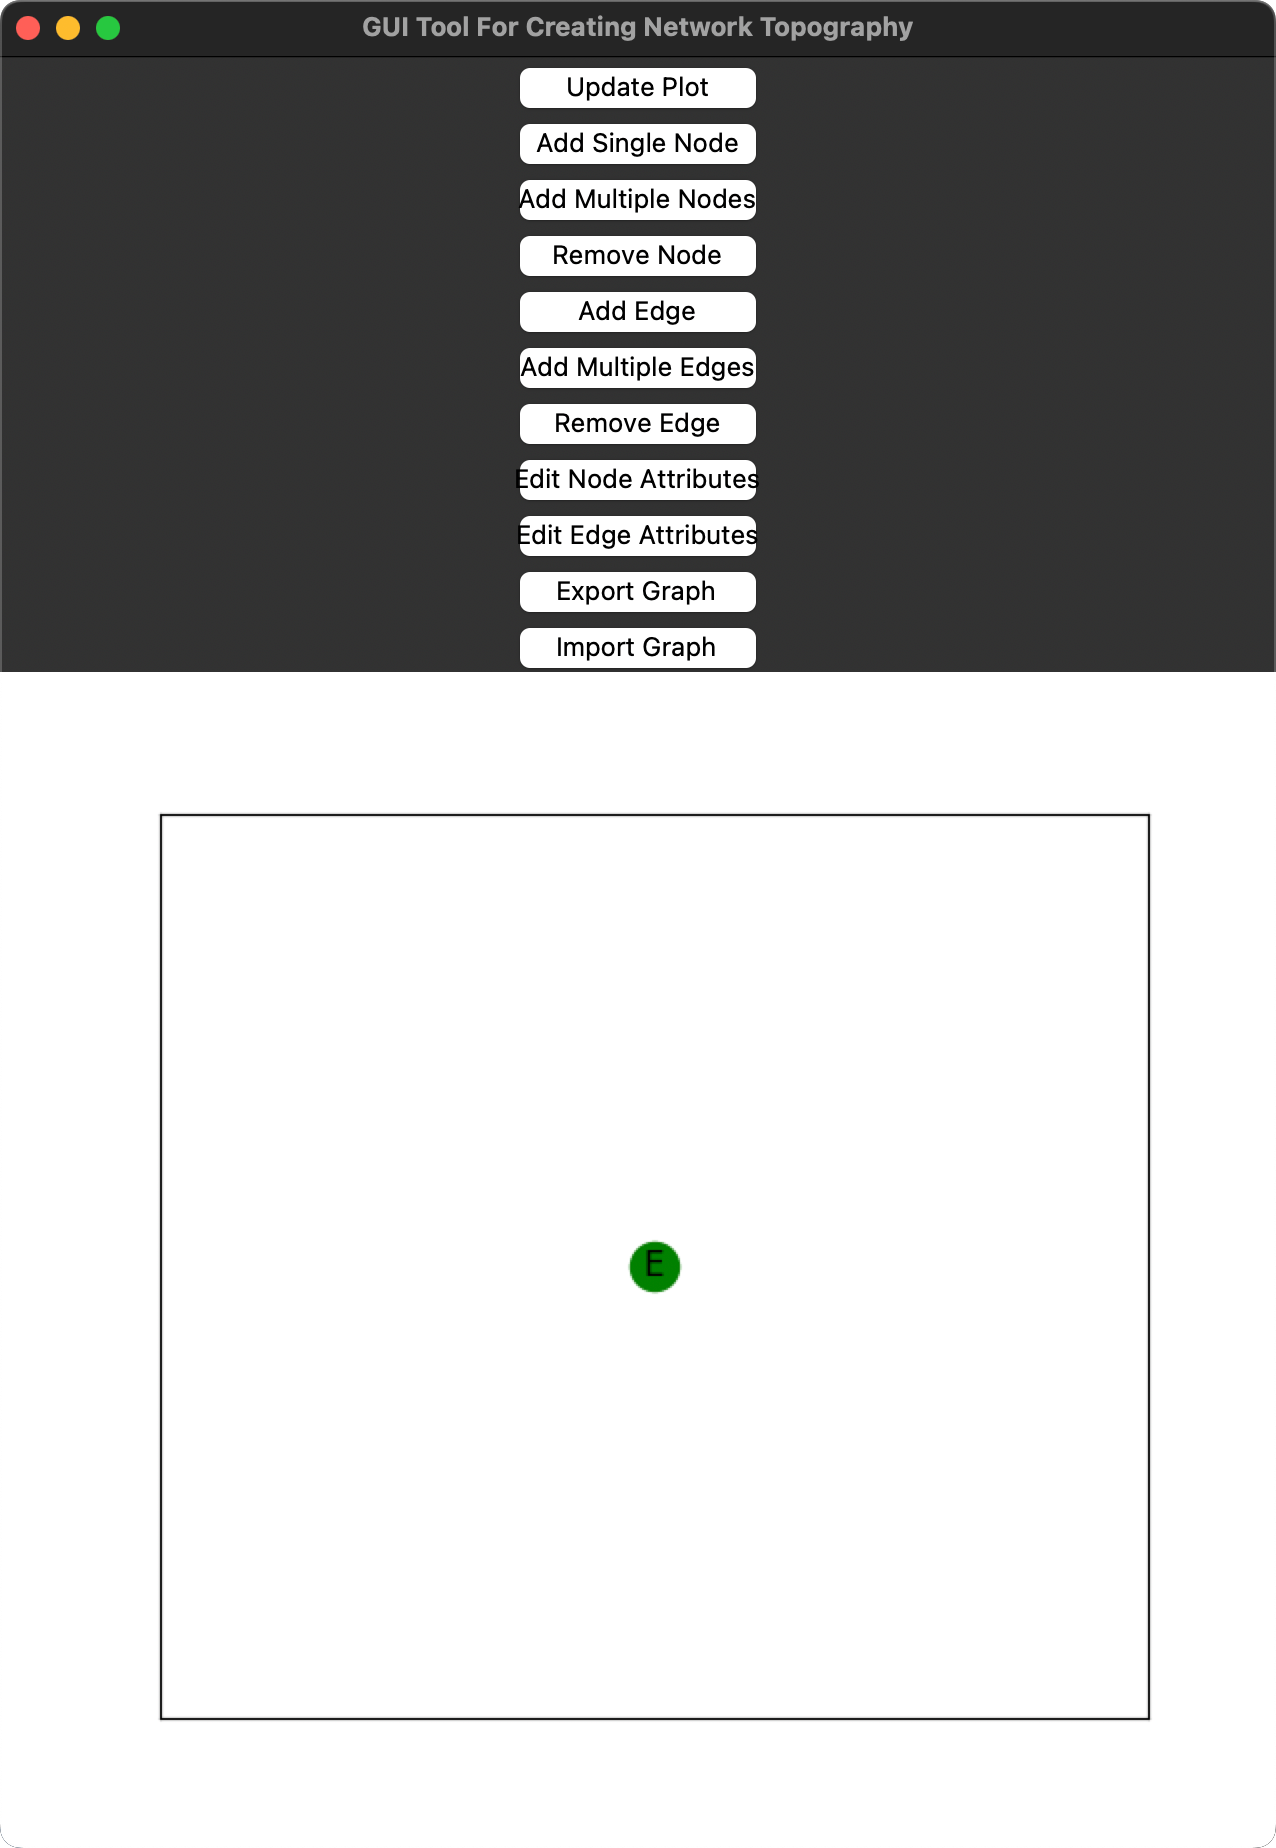
\includegraphics[width=\linewidth]{Screenshots/initial_startup_GUI_tool.png}
        \caption{
            The GUI tool as seen on the startup of the program.
        }
        \label{fig:ss:initial_startup_GUI_tool}
    \end{subfigure}
    \begin{subfigure}{0.49\linewidth}
        \centering
        \captionsetup{width=1\linewidth}
        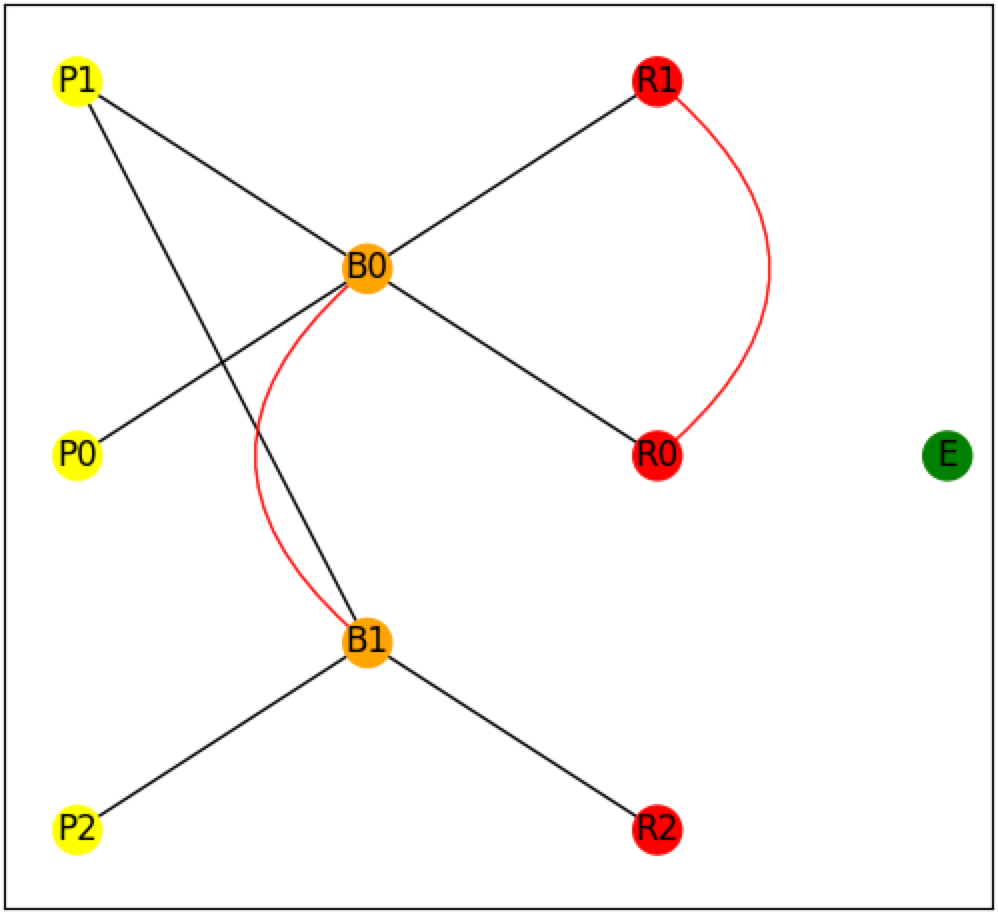
\includegraphics[width=\linewidth]{Screenshots/example_network.png}
        \caption{
            A $1\times1\times1$ and $2\times 2 \times 3$ network. 
        }
        \label{fig:ss:example_network}
    \end{subfigure} 
    \begin{subfigure}{0.49\linewidth}
        \centering
        \captionsetup{width=1\linewidth}
        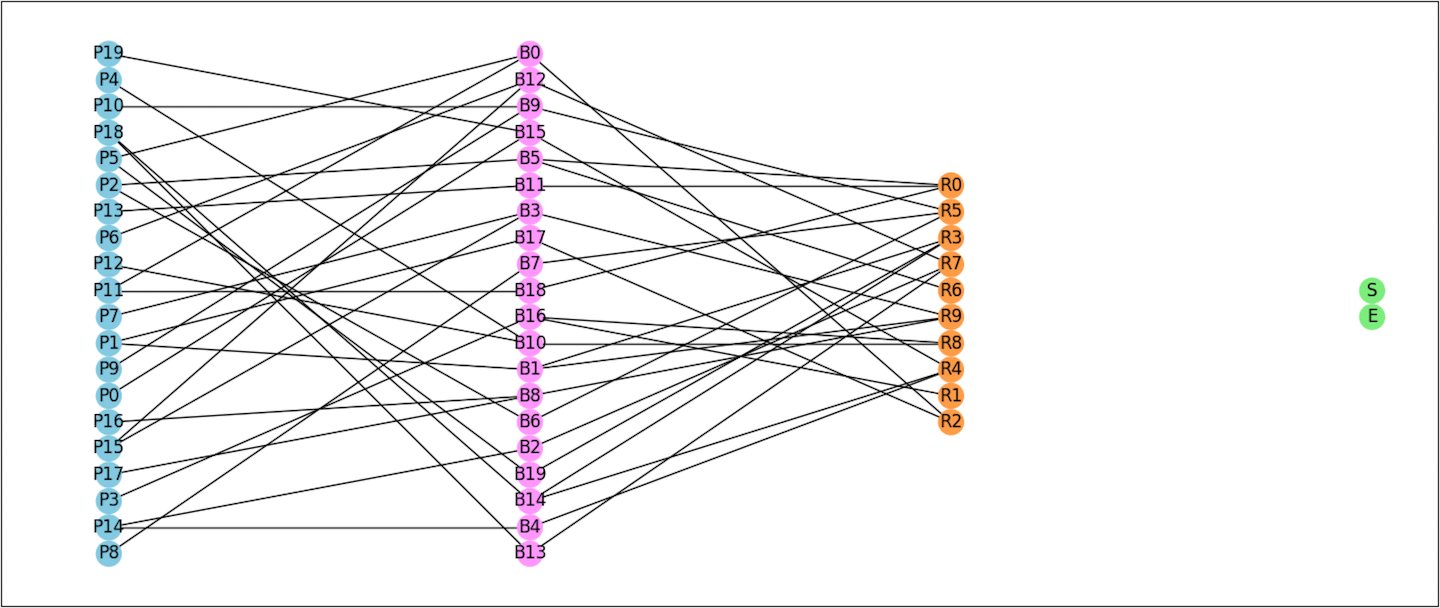
\includegraphics[width=\linewidth]{Screenshots/large_network.png}
        \caption{
            A $20\times20\times10$ network. 
        }
        \label{fig:ss:example_large_network}
    \end{subfigure} 
    \caption{
        This network topography along with a $1 \times 1 \times 1$ network will be used in the \Cref{Methods} and \Cref{AER} sections. 
            The parameter values for the networks can be found at \Cref{tab:appendixE:a_good_curve}, \Cref{tab:appendixE:complex_model} and \Cref{tab:appendixE:SOBOL_analysis_values}
        Each node represents a phage, bacteria, or resource, with arbitrary interactions occurring between them. 
        Although not shown and used here, edges between the same entity types and self loops are allowed. 
    }
    \label{fig:ss:GUI_tool_and_network}
 \end{figure}

\subsection{Simulation Framework} % TODO: Rewrite this section
\label{sec:simulation_framework}
The user provides an ODE model and the network topography as input to the framework. 
The simulation framework deals with handling the input, output, collecting and storing of the simulation input and output.
The framework uses SciPy's \cite{virtanenSciPy10Fundamental2020} \textit{solve\_ivp()} numerical solver \cite{ dormandFamilyEmbeddedRungeKutta1980} to simulate the provided ODE equations and calculate the population levels through time.
The user receives two outputs from the framework. 
The first output is an array of time values that the solver used to calculate the population count.
The second output is an array containing the population count at each time step for every entity.

In order to facilitate more complex model behavior, extra entities can be added to the simulation.  
Such an example would be the distinction between uninfected and infected bacteria. 
In the network model you explicitly create a $3\times 2 \times 3$ network, with 3 phages, 2 bacteria, and 3 resources. 
You explicitly tell the solver to add $2\cdot M$ additional states that represent the infected states. 
So the ODE solver would solve for 3 phages, 2 uninfected bacteria states, $2\cdot M = 2\cdot 4=8$ infected bacteria states, and 3 resources. 

Adding a resource reservoir to the model would be simple as well. 
3 extra resource entities would be added to the system, where the resources would model the transfer of resources from the reservoir to the simulation environment. 
The provided ODE model will have to correctly model and transfer the resources from $R_{r_{\text{reservoir}}}$ to $R_{r_{\text{chemostat}}}$. 
The bacteria would only consume from $R_{r_{\text{chemostat}}}$. 

The user's ODE model has to correctly model each (extra) entity and correctly handle the changes in states. 

\subsection{Visualization Dashboard}
\label{sec:visualization_framework}
The third part involves analyzing and visualizing the simulation results on an interactive Dash Plotly \cite{DashDocumentationUser} dashboard. 
The user can use a dashboard built using Plotly Dash to interact with the solver and network.
The user can quickly change parameter, environment, and setting values with the dashboard. 
As output, the dashboard will show interactive plots so that the user can analyze the system. 

The dashboard allows the user to interact with the network, the model, and some prebuilt visualizations, and is built into three logical sections.
The first section allows for the user to edit the network parameters and setting values on the fly to quickly iterate through different conditions and to fine-tune parameter selection without having to rebuild the network using the GUI tool.
The second section allows for the user to see how the population count evolves over time for a given IC and parameter values, allowing to quickly test the network input.
The final section allows for the user to run more advanced analyses on the network, for example, by changing multiple parameter values and visualizing the output. 

\subsubsection{Editing Network and Parameter Values}
\label{sec:editing_network_and_parameter_values}
The editing network and parameter value contain five separate sections.
\paragraph{Initial Condition}
The IC settings panel (\Cref{fig:ss:ds:initial_condition}) allows the user to edit the initial starting values of the entities. 
Each entity type has a table containing the initial population count. 
\paragraph{Vector Data} 
Data that can be represented as a vector have their own section. 
This data would typically be seen with node data. 
So the washin rate of resources, or how fast a bacteria goes through the infection stage would be represented as a vector \Cref{fig:ss:ds:vector}.
\paragraph{Matrix Data}
Data that is stored as a matrix, the data stored on edges between entities, is stored in the matrix tab, \Cref{fig:ss:ds:matrix}.
This would typically be data that is stored on the edges, for example the phage infection speed or how fast a bacteria can consume a resource. 
\paragraph{Environment and settings}
The environment data and settings data also have their own tab, \Cref{fig:ss:ds:environment} and \Cref{fig:ss:ds:settings} respectively. 
The data stored in the environment act as global variables, like the pH of the system, or the constant washout rate. 
THe settings node holds the solver and simulation settings like the length of the simulation or minimum time-step. 

\begin{figure}[h!]
    \centering
    \begin{subfigure}{0.49\linewidth}
        \centering
        \captionsetup{width=1\linewidth}
        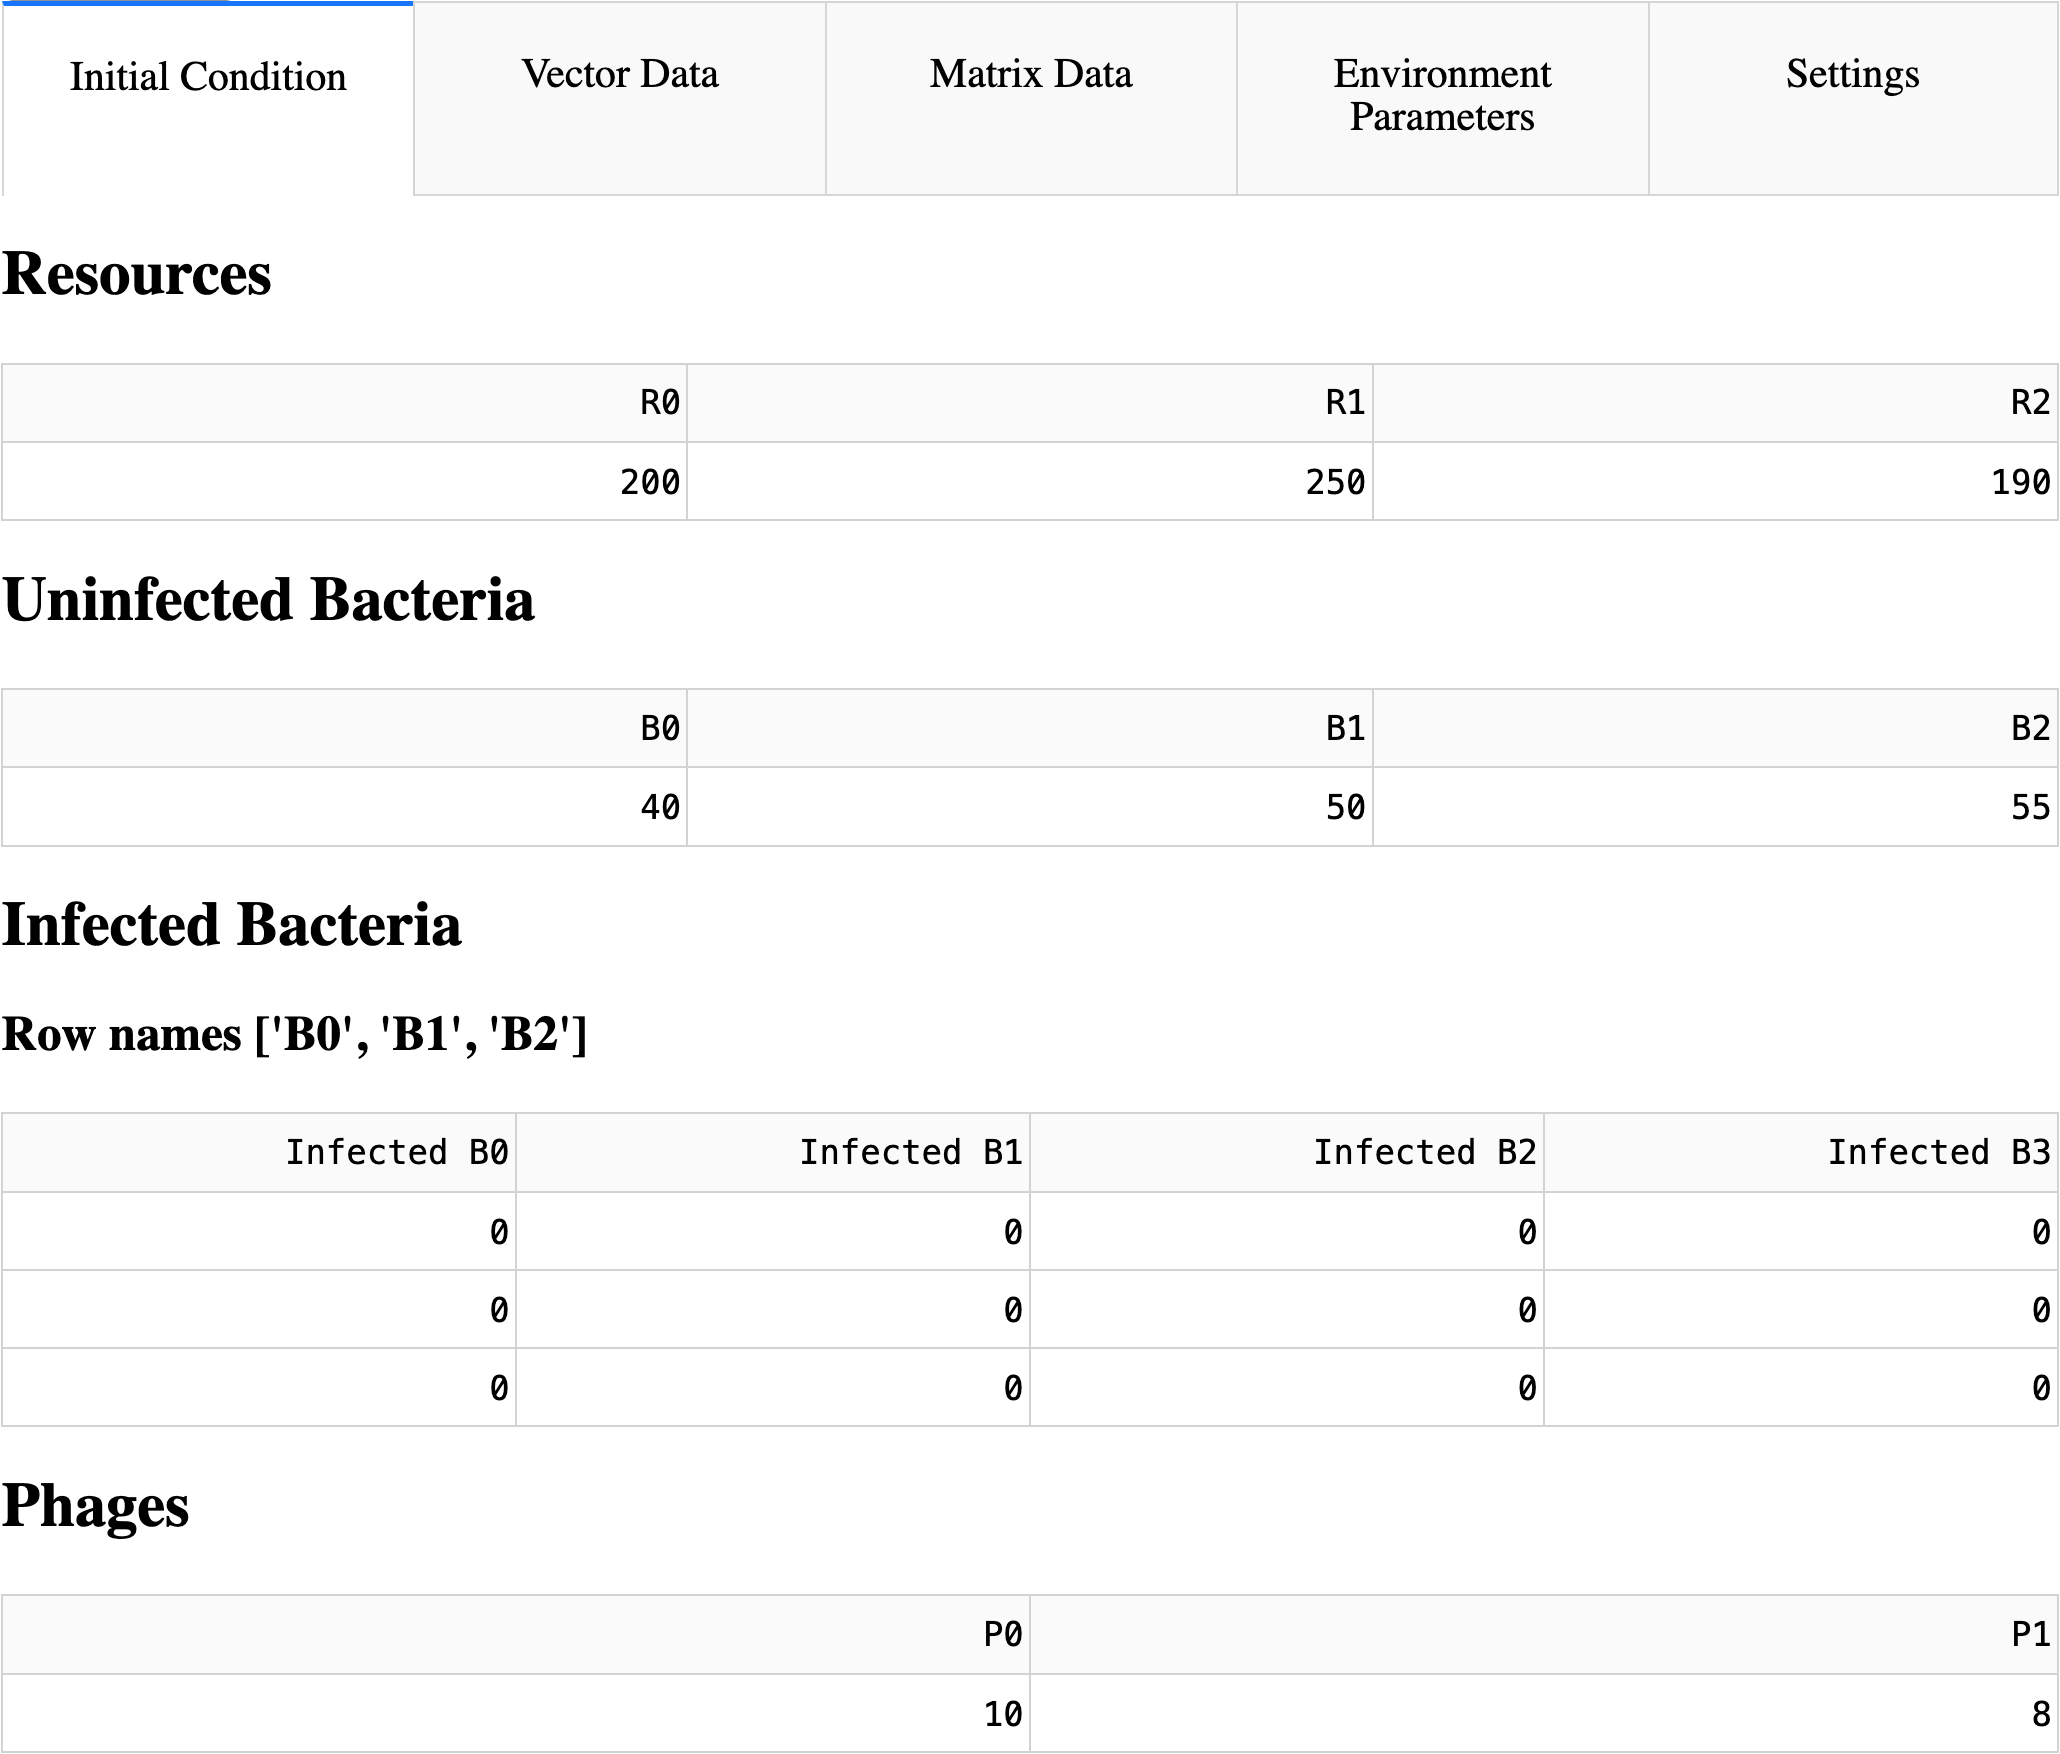
\includegraphics[width=\linewidth]{Screenshots/DashboardSettings/initial_condition_settings.png}
        \caption{
            The tab where the user can edit the ICs of the entities.
        }
        \label{fig:ss:ds:initial_condition}
    \end{subfigure}
    \hfill
    \begin{subfigure}{0.49\linewidth}
        \centering
        \captionsetup{width=1\linewidth}
        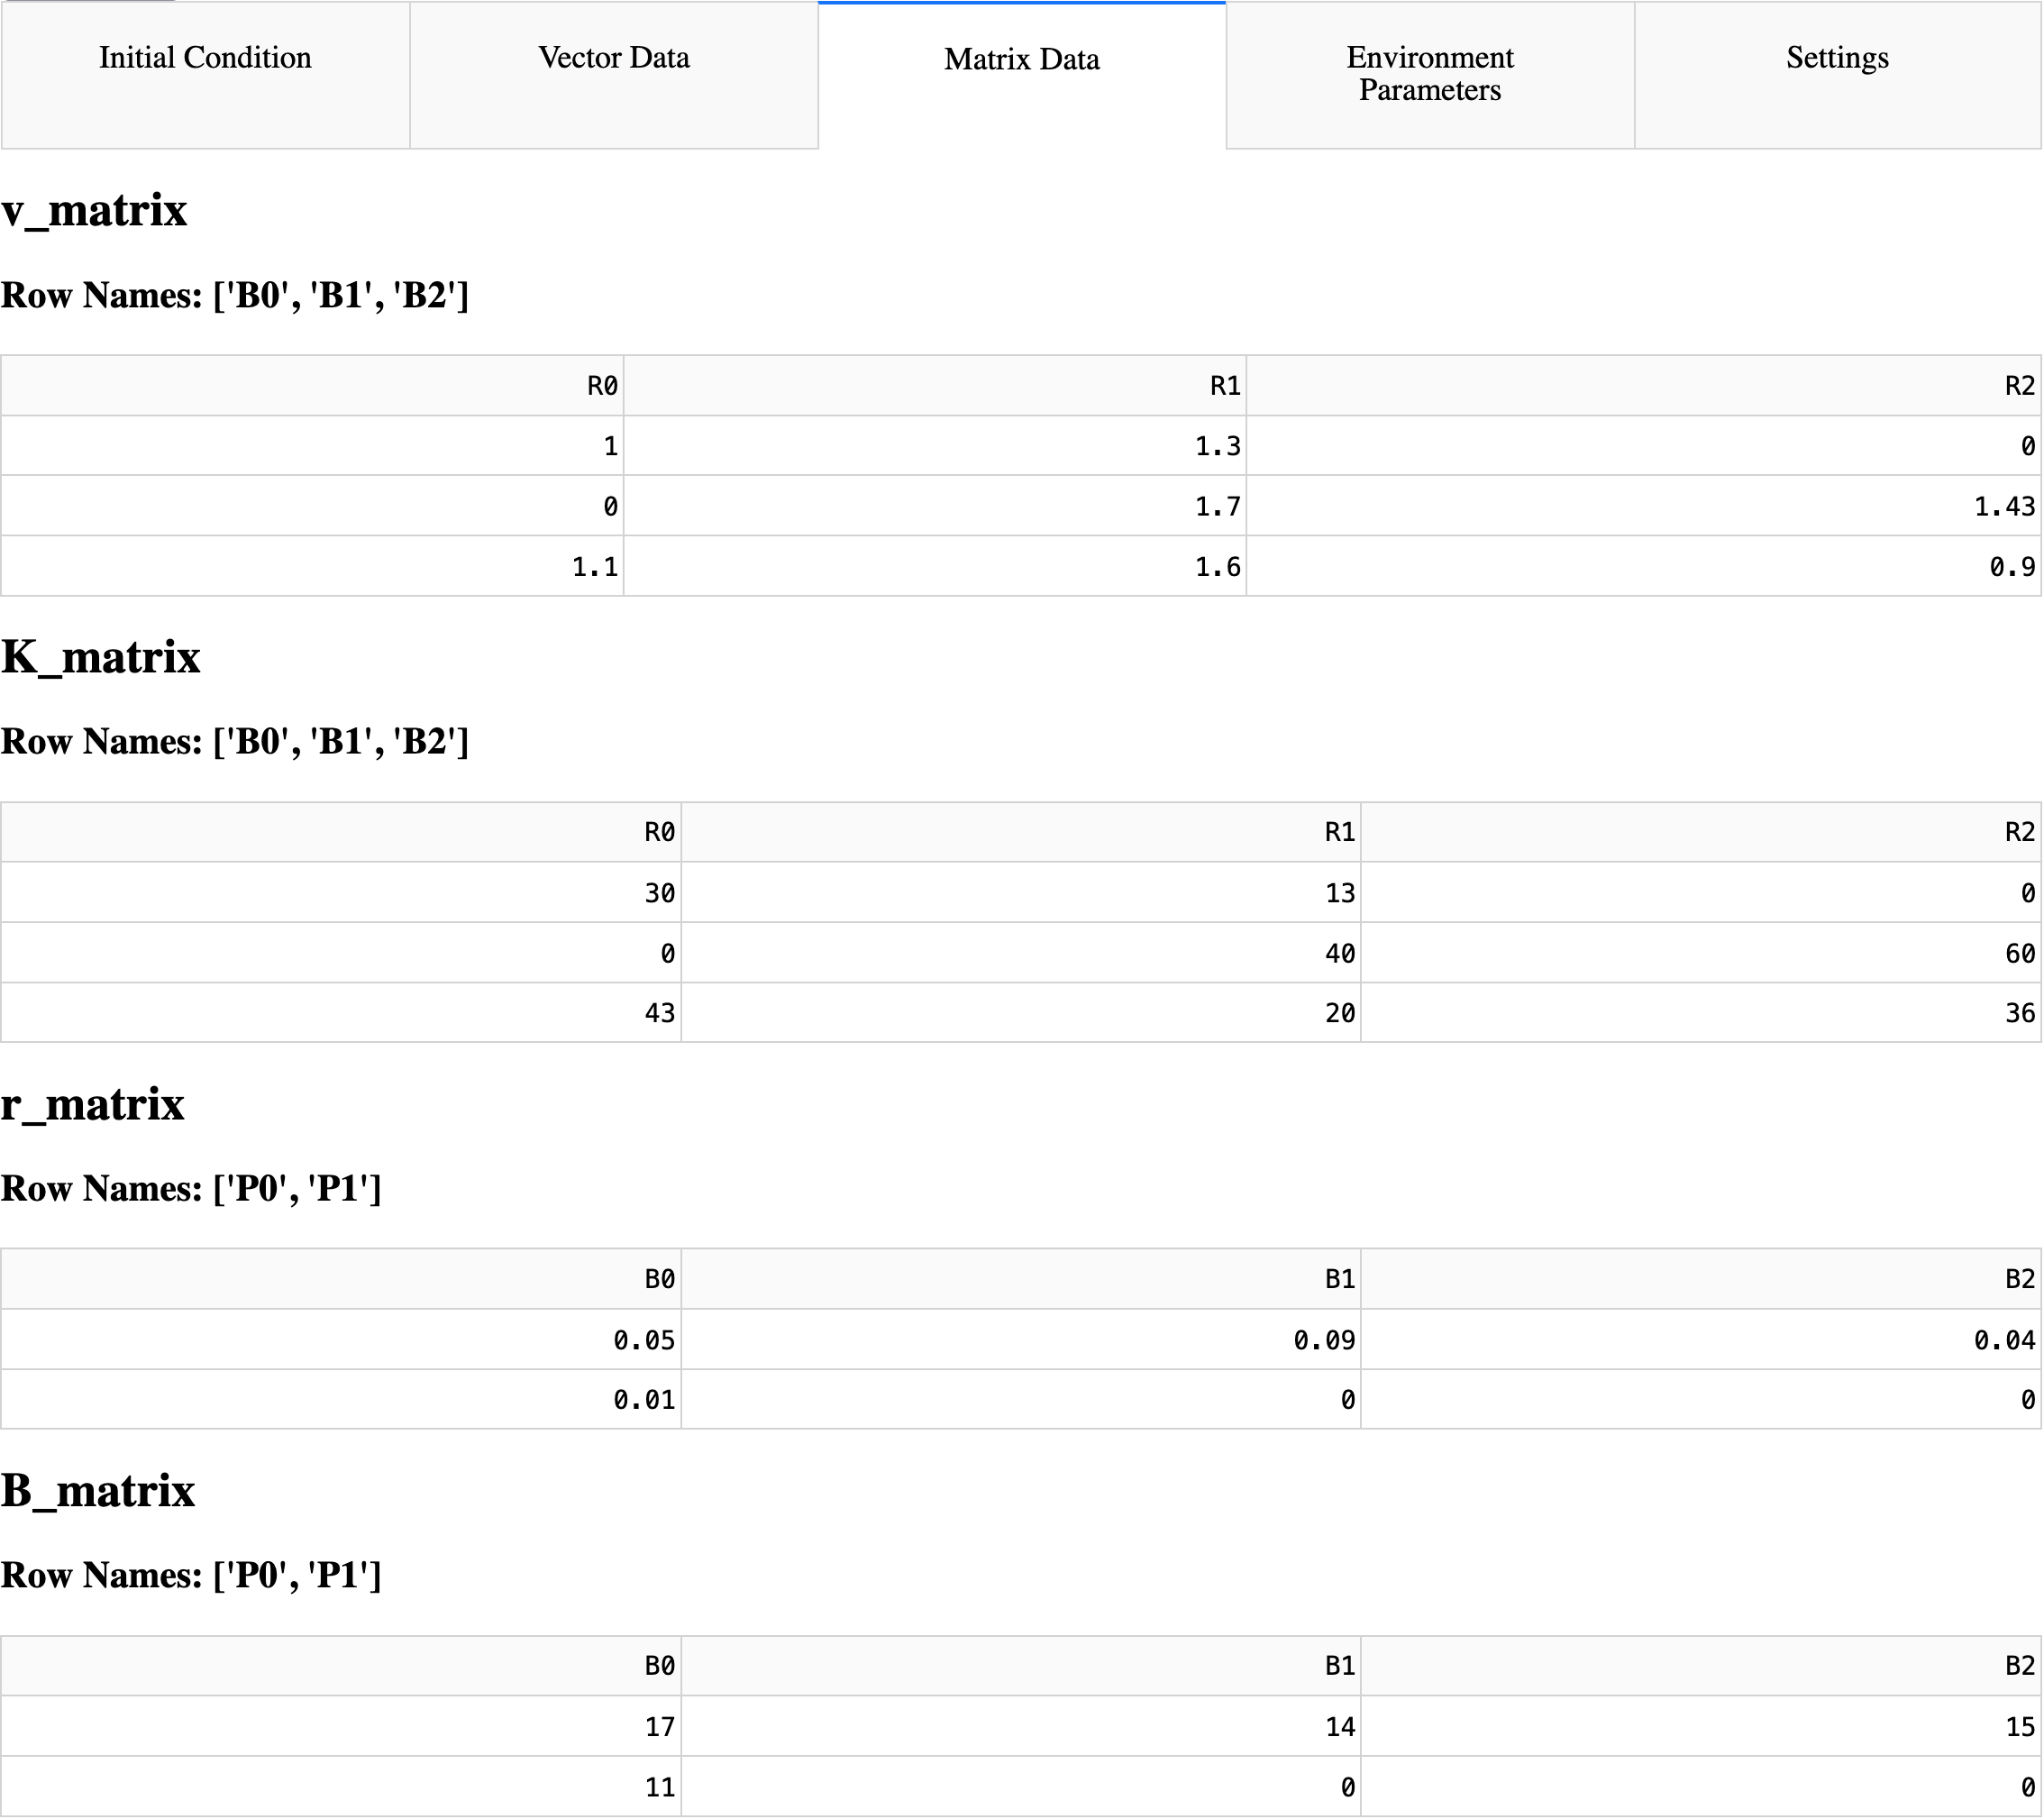
\includegraphics[width=\linewidth]{Screenshots/DashboardSettings/initial_matrix_settings.png}
        \caption{
            The tab where the user can edit the matrix attribute values. 
        }
        \label{fig:ss:ds:matrix}
    \end{subfigure}
    \hfill
    \begin{subfigure}{0.49\linewidth}
        \centering
        \captionsetup{width=1\linewidth}
        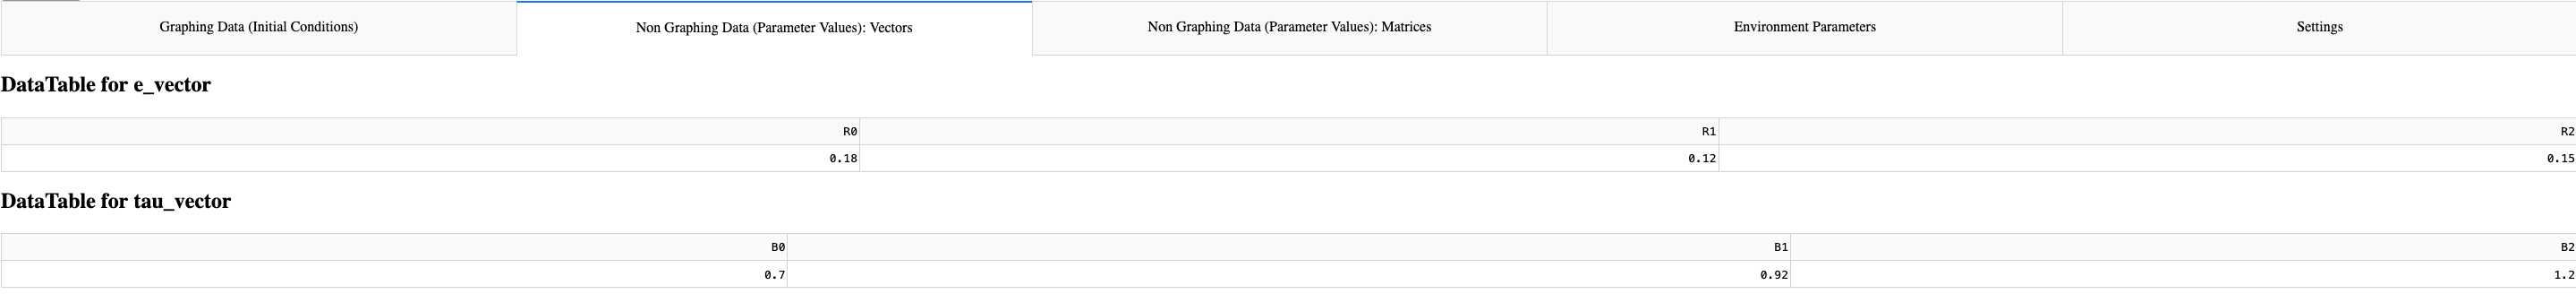
\includegraphics[width=\linewidth]{Screenshots/DashboardSettings/initial_vector_settings.png}
        \caption{
            The tab where the user can edit the vector attribute values.
        }
        \label{fig:ss:ds:vector}
    \end{subfigure}
    \hfill
    \begin{subfigure}{0.49\linewidth}
        \centering
        \captionsetup{width=1\linewidth}
        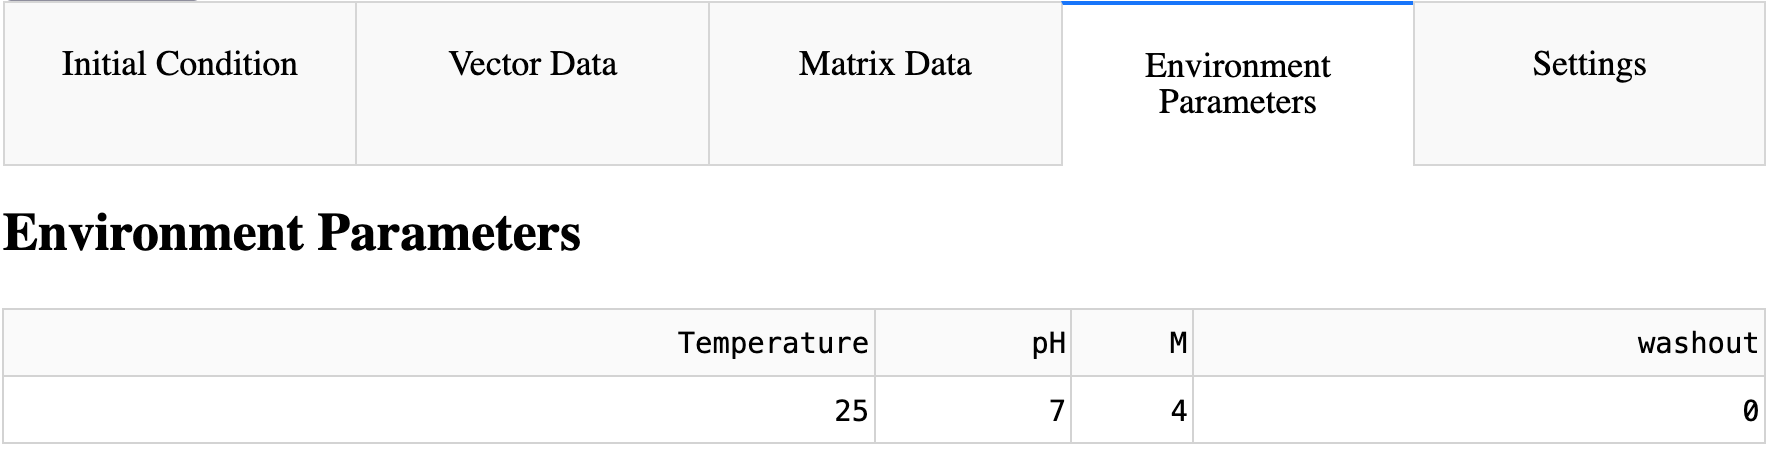
\includegraphics[width=\linewidth]{Screenshots/DashboardSettings/initial_environment_settings.png}
        \caption{
            The tab where the user can edit the environment values. 
        }
        \label{fig:ss:ds:environment}
    \end{subfigure}
    \hfill
    \begin{subfigure}{0.49\linewidth}
        \centering
        \captionsetup{width=1\linewidth}
        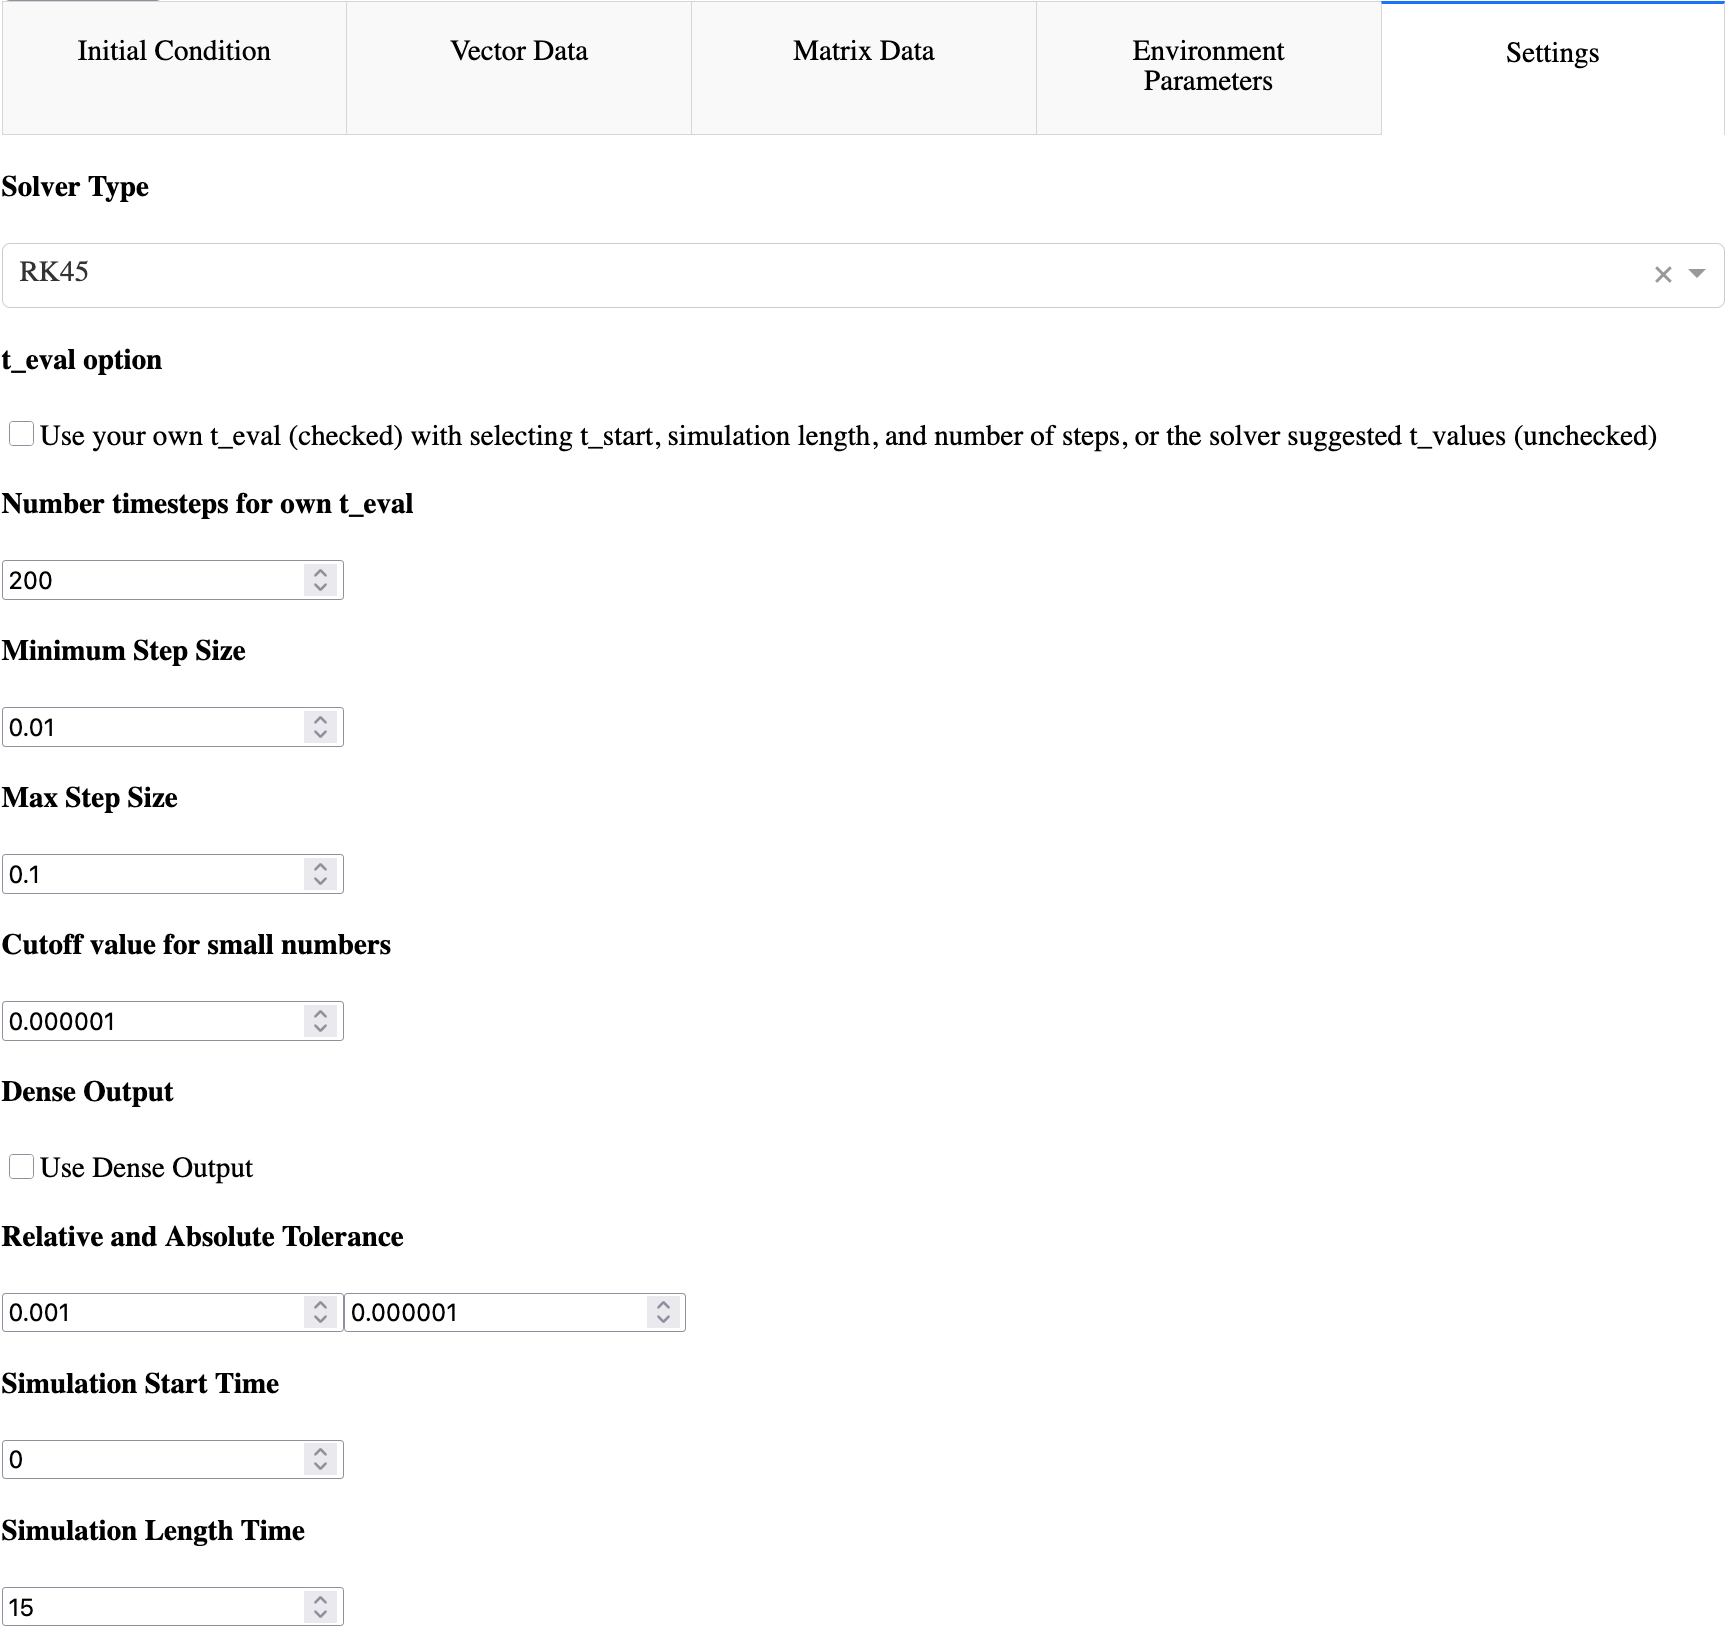
\includegraphics[width=\linewidth]{Screenshots/DashboardSettings/initial_settings_settings.png}
        \caption{
            The tab where a user can edit the settings of the solver and simulation. 
        }
        \label{fig:ss:ds:settings}
    \end{subfigure}
    \caption{The tabs where the user can edit the various parameter values and control the simulation parameters}
 \end{figure}

\subsubsection{Visualization and Analysis}
In the analysis section, the user can run different analysis methods to gain a greater understanding of the model.
For simplicity, the visualizations on the dashboard only support a $1 \times 1\times 1$ model. 
This makes it easier for the user to analyze the system. 
The goal of the dashboard is to investigate a simple system in order to gain a deeper understanding of the system. 
There are five prebuilt visualizations which are described below. 
These five visualizations are called serial transfer, parameter analysis, initial value analysis, serial trasnfer, and SOBOL analysis. 
The aim of the visualizations is to investigate how the system changes with respect to varying inputs. 

After the user has a deeper understanding of the system, they can run and download custom simulations to create their own custom visualizations in the Ultimate Analysis section. 
The saved simulation data is stored as a \textit{.parquet} file, a tabular-like data format. 
The simulation data can be queried with Dask, allowing a user to find a specific simulation result. 
Parquet with Dask offers superior performance and data storage solutions that Pandas doesn't offer.

\paragraph{Serial Transfer}
\label{sec:serial_transfer}
On the dashboard, a user can select the dilution factor which will divide the population count of the phages, bacteria, and resources by that number (\Cref{fig:ss:av:serial_transfer_settings}).
Then the program takes the IC values defined in \Cref{sec:editing_network_and_parameter_values} and adds those values to the respective entity. 

As an example, if the simulation ended with 3500 phages, 100 (uninfected) bacteria and 50 resources, the dilution factor is 10, and the user wants to add 350 new bacteria and 130 new resources for the next simulation, the new starting condition for the next simulation would be $\frac{3500}{10} = 350$ phages, $\frac{100}{10} + 350 = 660$ bacteria, and $\frac{50}{10} + 130 = 135$ resources.

As output, ST will show how the population evolved through time as well as the final population value at the end of each serial transfer run. 
An example output is shown in \Cref{fig:ss:av:serial_transfer_run}.

\begin{figure}[h!]
    \centering
    \begin{subfigure}{0.49\linewidth}
        \centering
        \captionsetup{width=1\linewidth}
        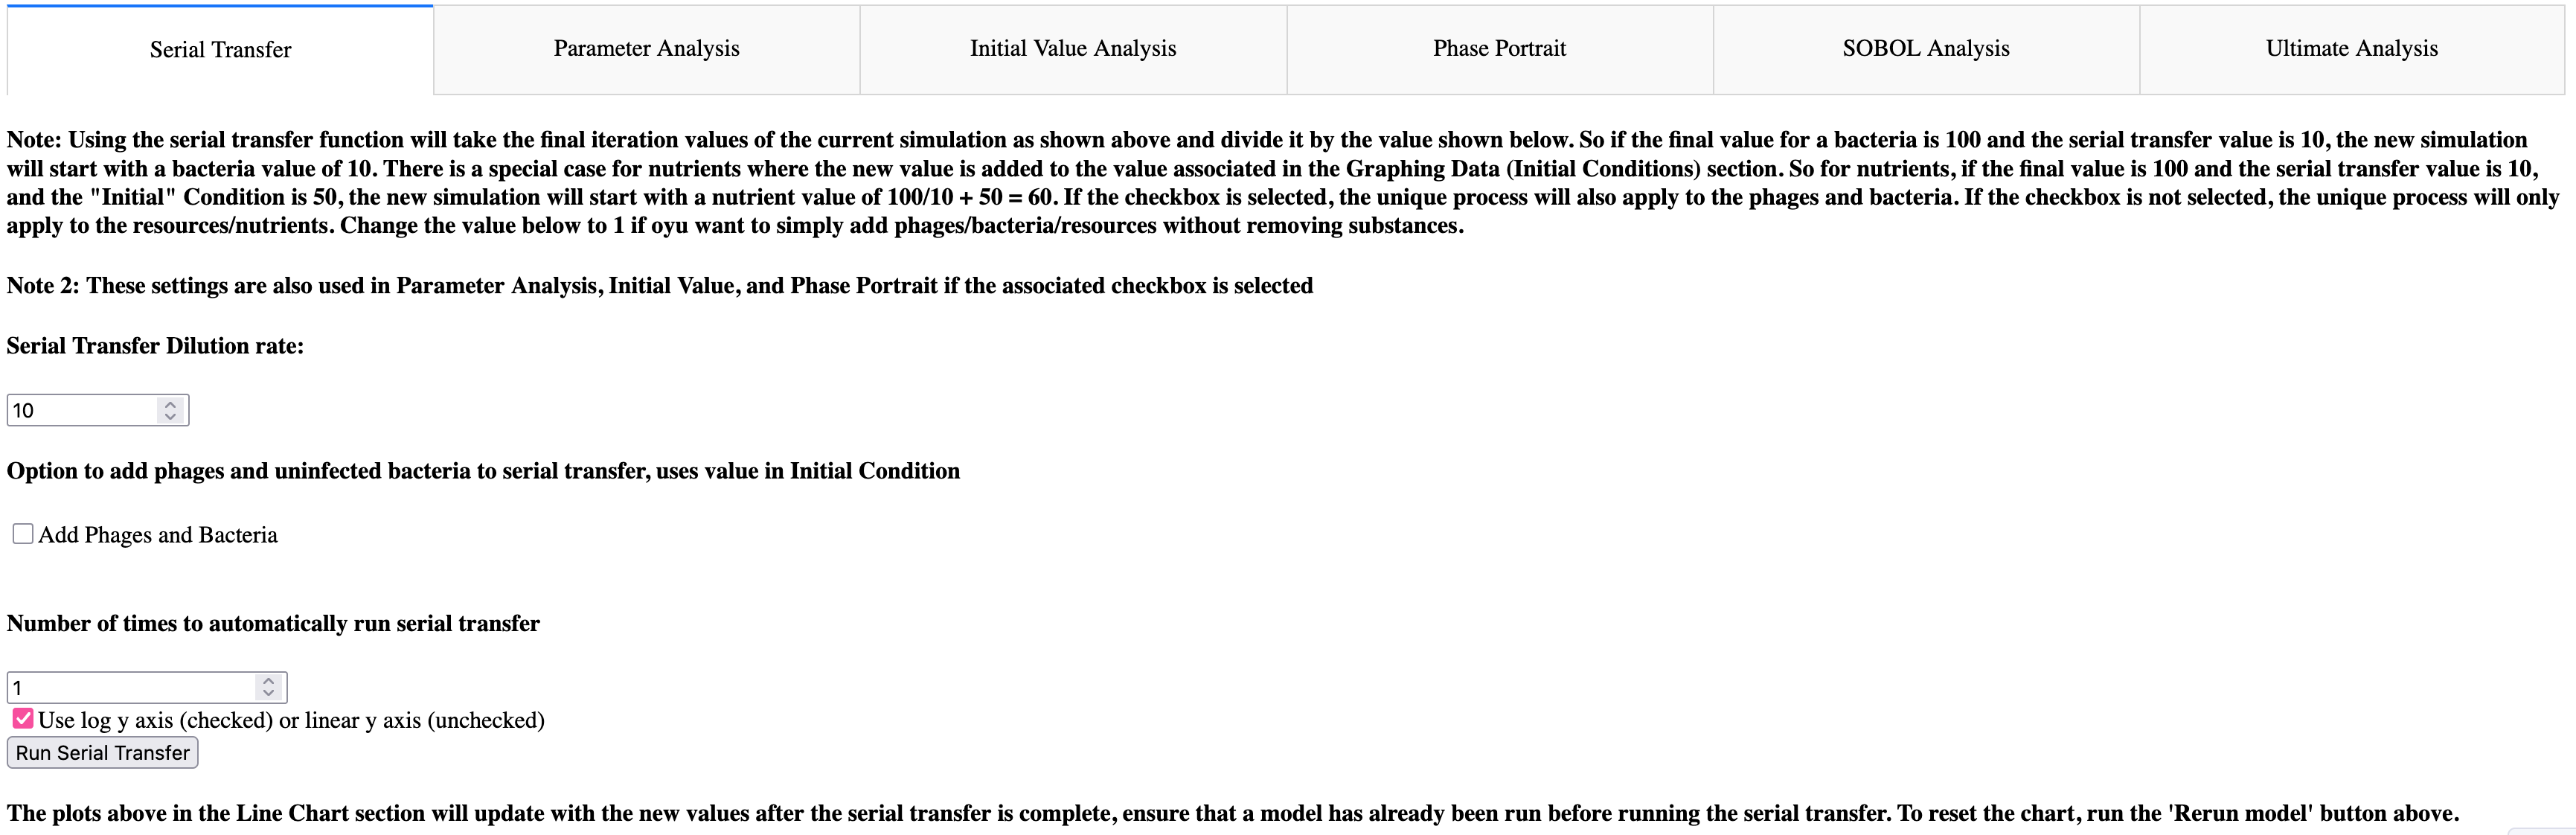
\includegraphics[width=\linewidth]{Screenshots/AdvancedVisualization/serial_transfer_settings.png}
        \caption{
            The section where the user can set up the ST.
        }
        \label{fig:ss:av:serial_transfer_settings}
    \end{subfigure}
    \hfill
    \begin{subfigure}{0.49\linewidth}
        \centering
        \captionsetup{width=1\linewidth}
        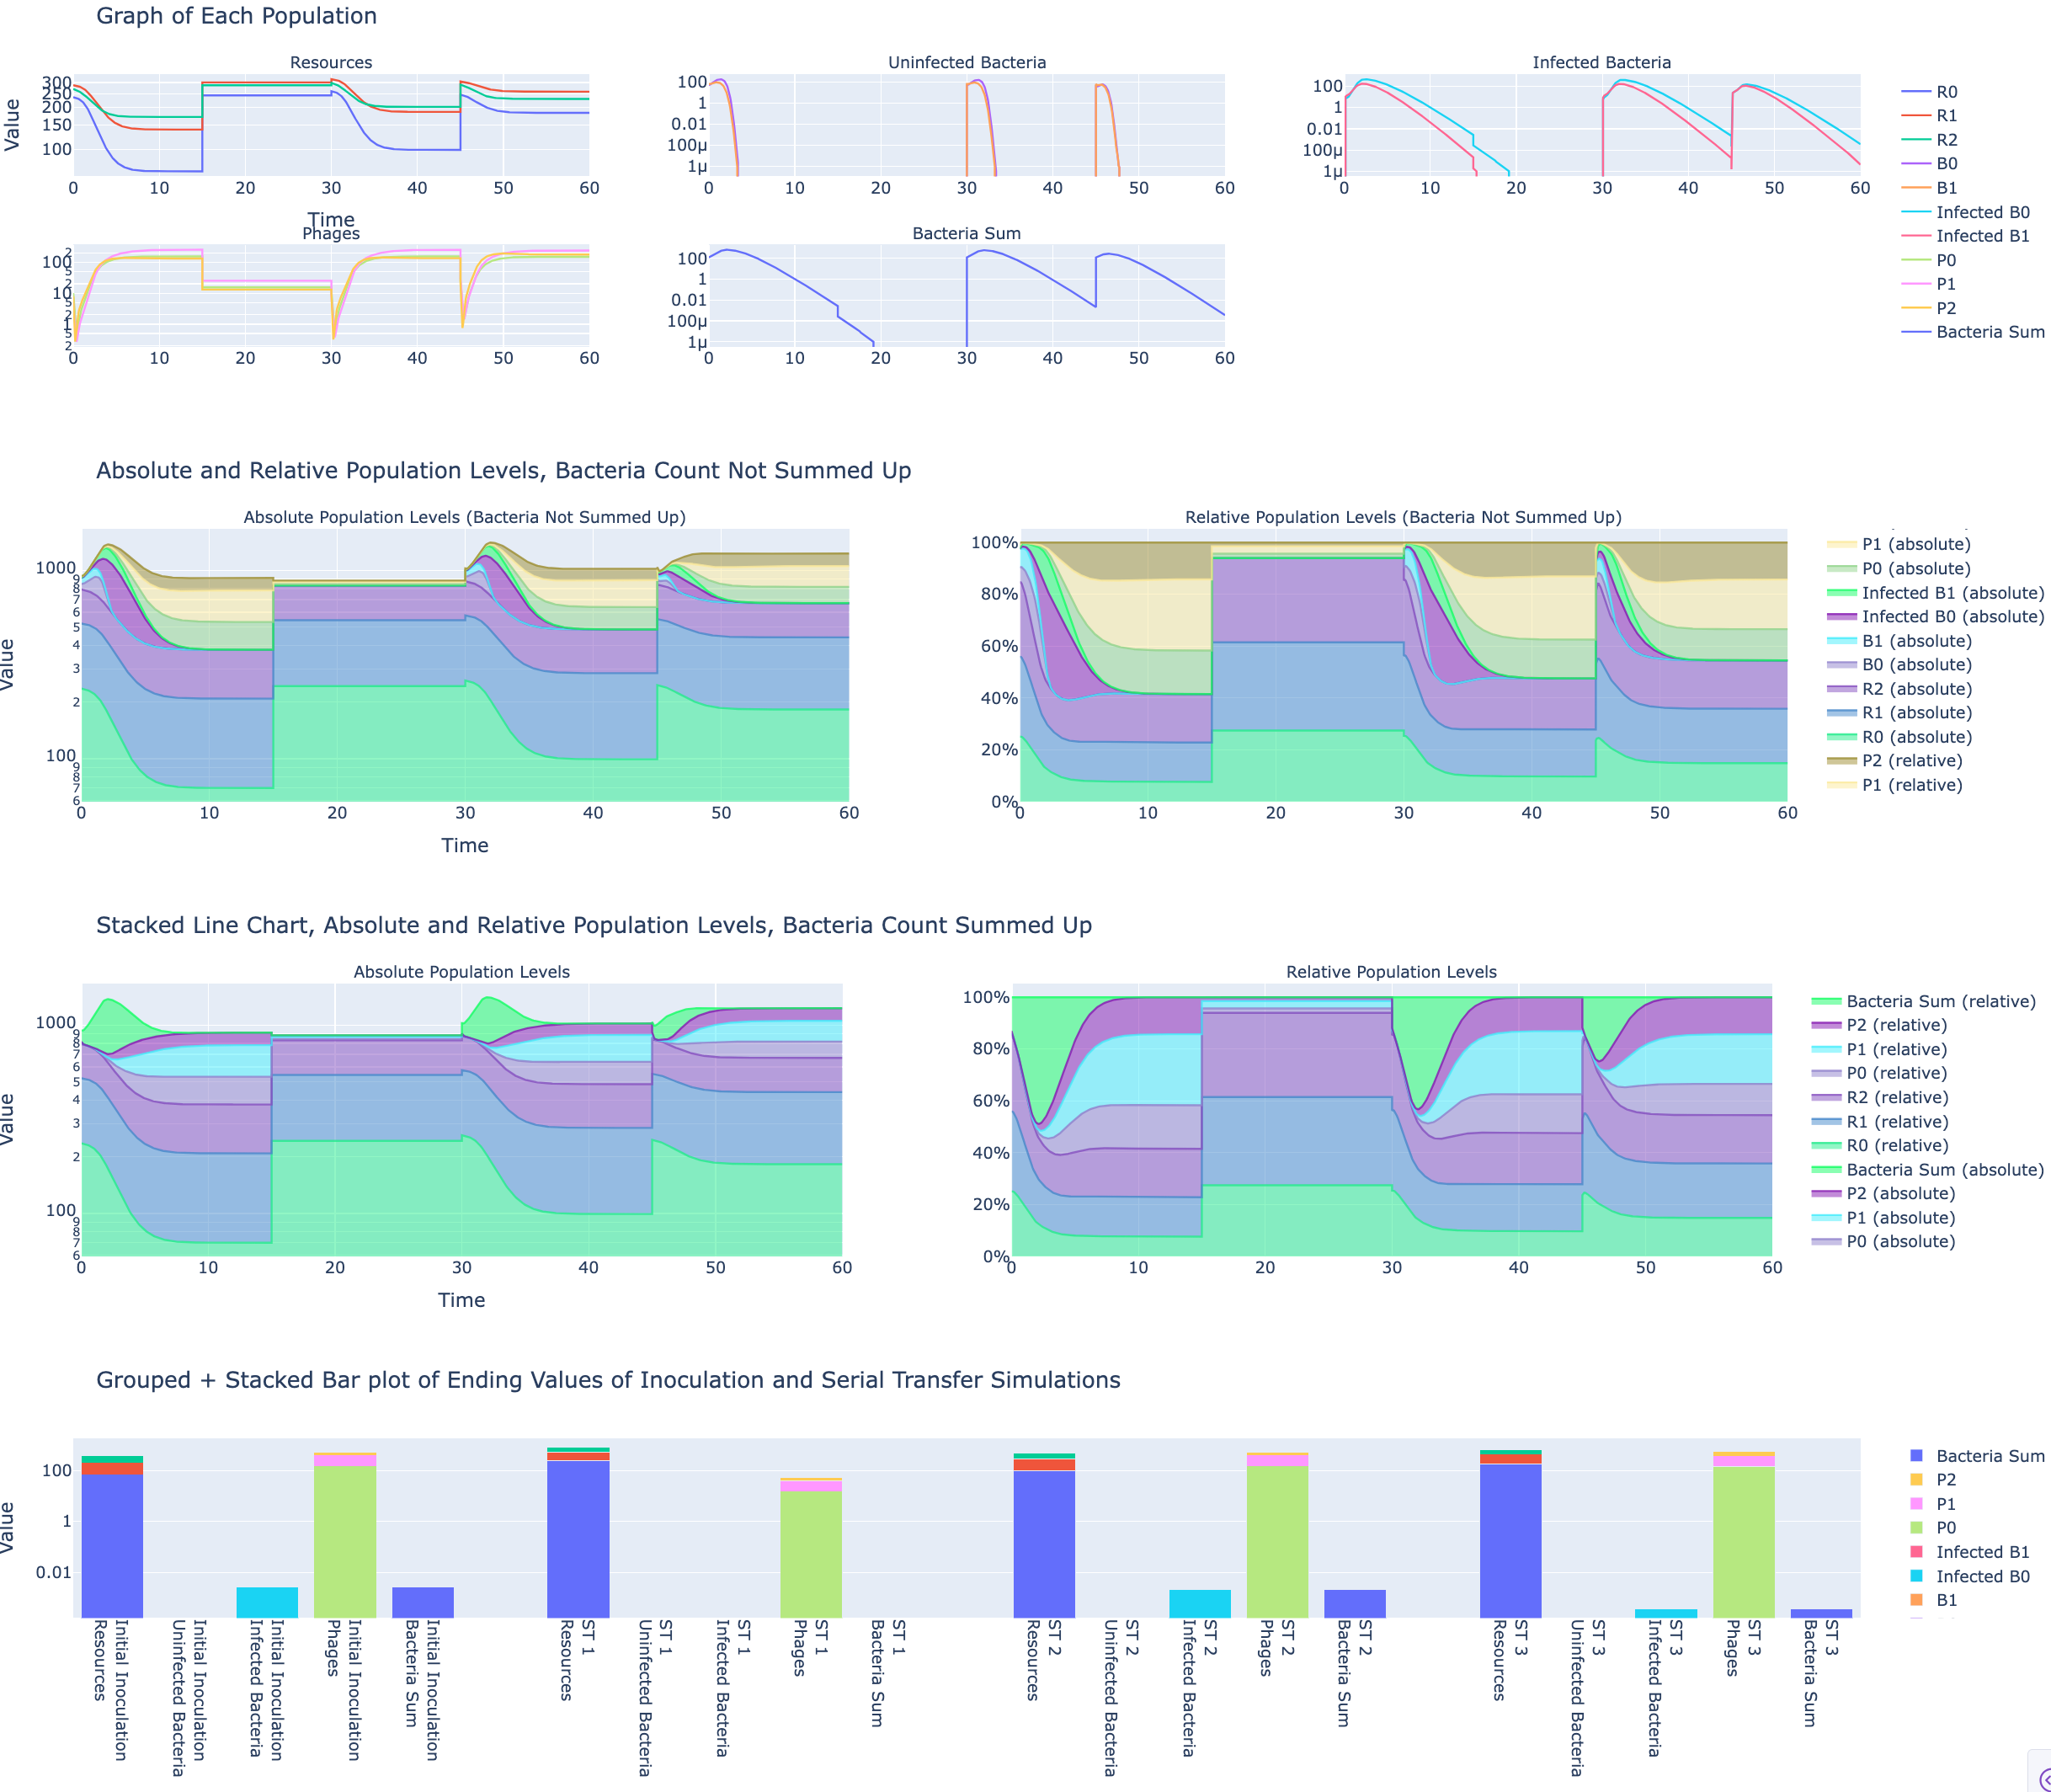
\includegraphics[width=\linewidth]{Screenshots/AdvancedVisualization/serial_transfer_run.png}
        \caption{
            The ST output plots. 
        }
        \label{fig:ss:av:serial_transfer_run}
    \end{subfigure}
    \caption{Serial Transfer}
 \end{figure}

\paragraph{Parameter Analysis}
\label{sec:parameter_analysis}
The parameter analysis (PA) settings tab as shown in \Cref{fig:ss:av:parameter_analysis_settings} allows the user to choose two parameters and individually run the model with the varying input values.
The values that can be tested and changed include all IC values, vector and matrix data, and environmental data.
As input, the user can select 2 parameters of choice.
After the parameter name selection, the user can manually choose which parameter values they want to test or test a range of values equally spaced by selecting the number of values to test.
Finally, the user can optionally run a ST, where the ST uses the settings found on the ST tab. 

\Cref{fig:ss:av:parameter_analysis_run} shows the heatmap that the user can expect, one heatmap for each entity type.
Each heatmap cell represents the input of 2 unique parameter values, and shows the population count for that parameter run at the time shown in the slider. 
As the user slides the slider, the value inside the cell updates to correspond with the selected time. 
Note that the heatmap color range resets for each heatmap, so similar colors across heatmaps and across time will not correspond to the same values.

\begin{figure}[h!]
    \centering
    \begin{subfigure}{0.49\linewidth}
        \centering
        \captionsetup{width=1\linewidth}
        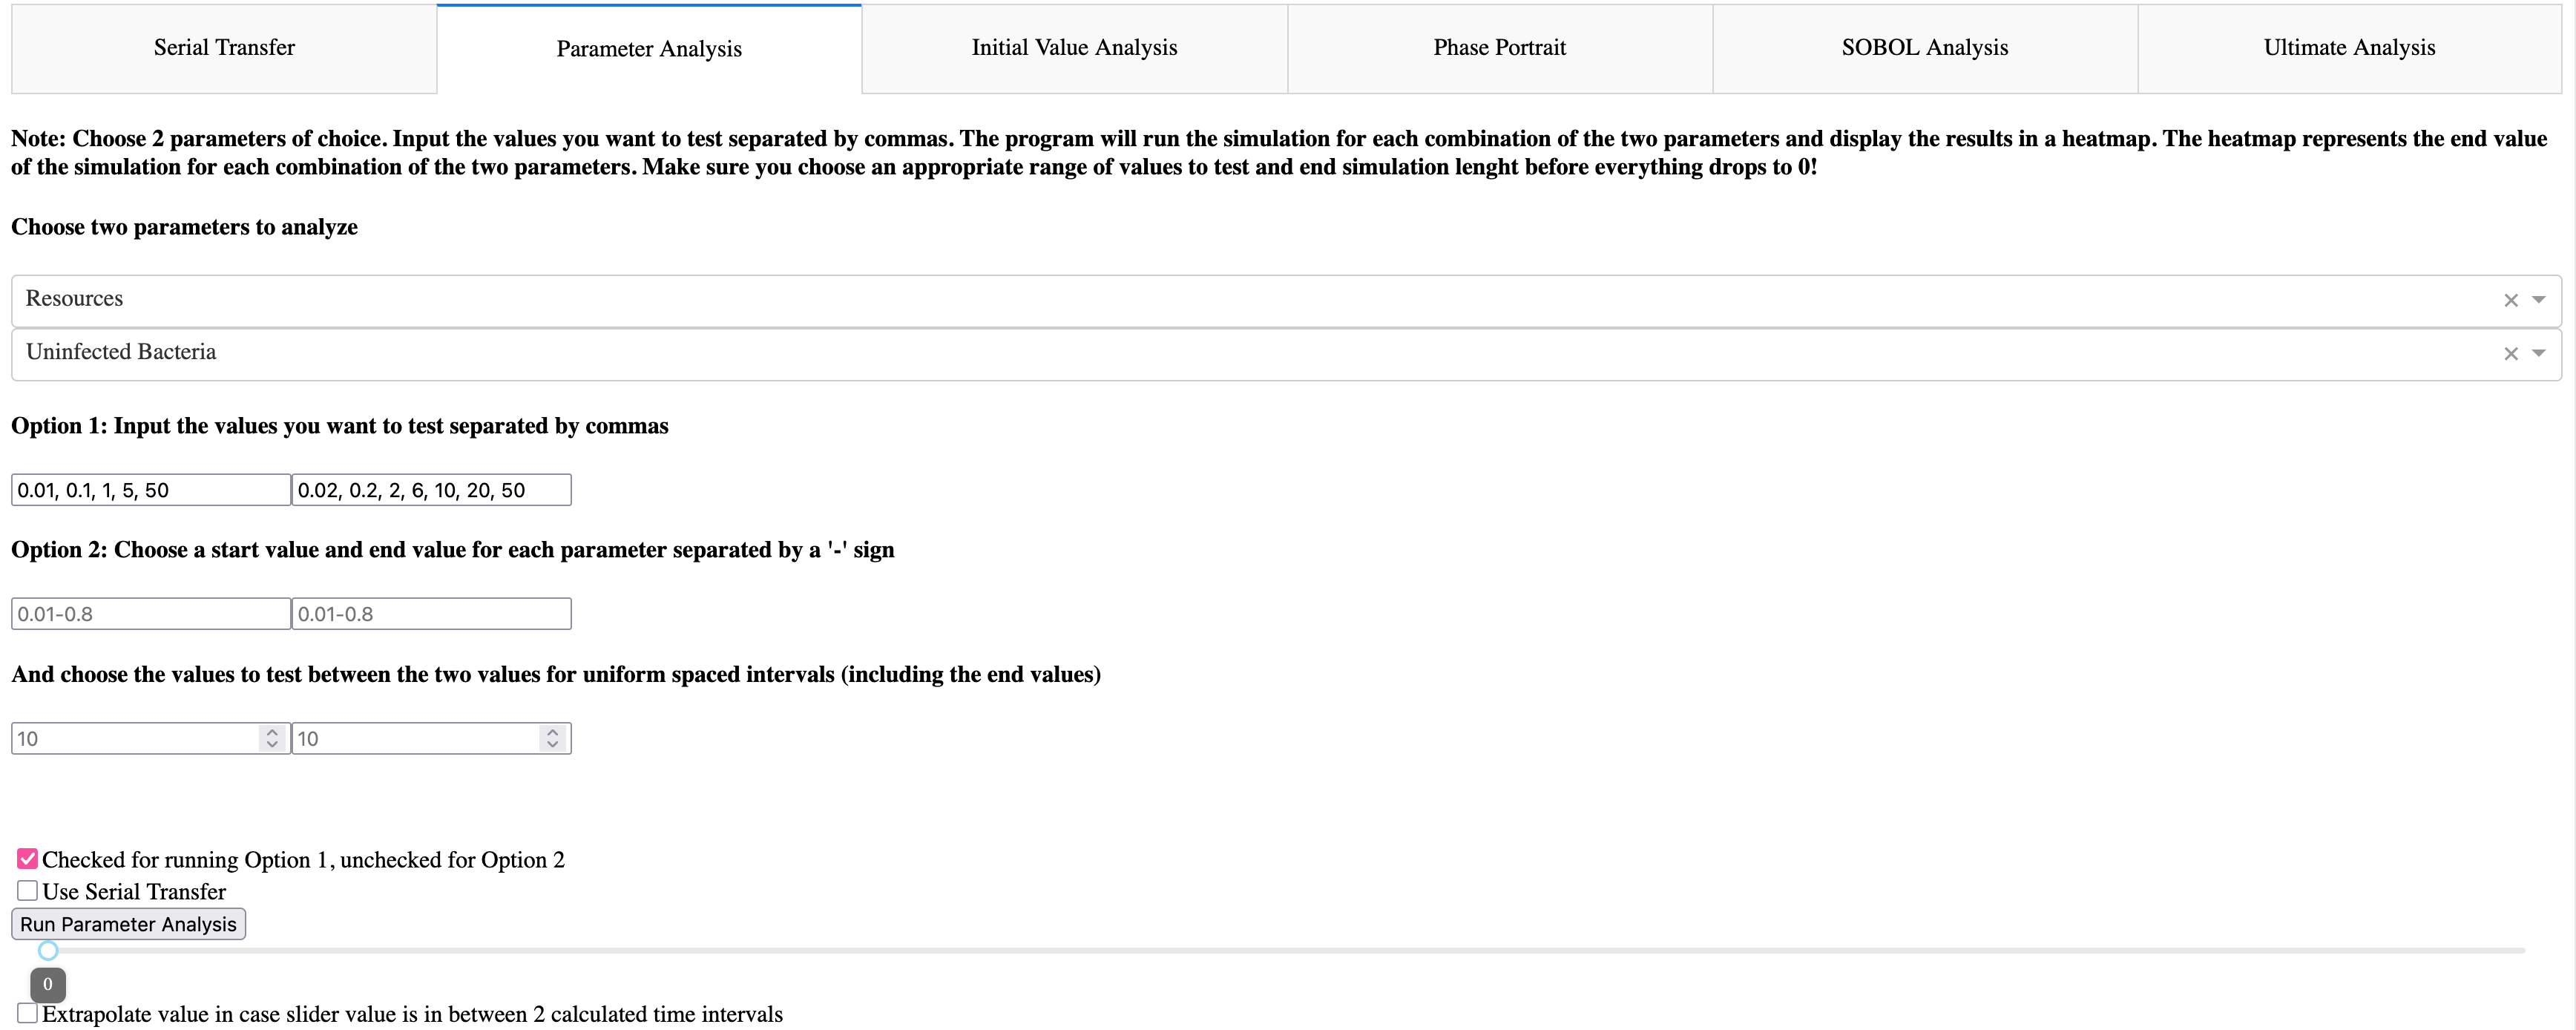
\includegraphics[width=\linewidth]{Screenshots/AdvancedVisualization/parameter_analysis_settings.png}
        \caption{
            The available phase portrait settings. 
        }
        \label{fig:ss:av:parameter_analysis_settings}
    \end{subfigure}
    \hfill
    \begin{subfigure}{0.49\linewidth}
        \centering
        \captionsetup{width=1\linewidth}
        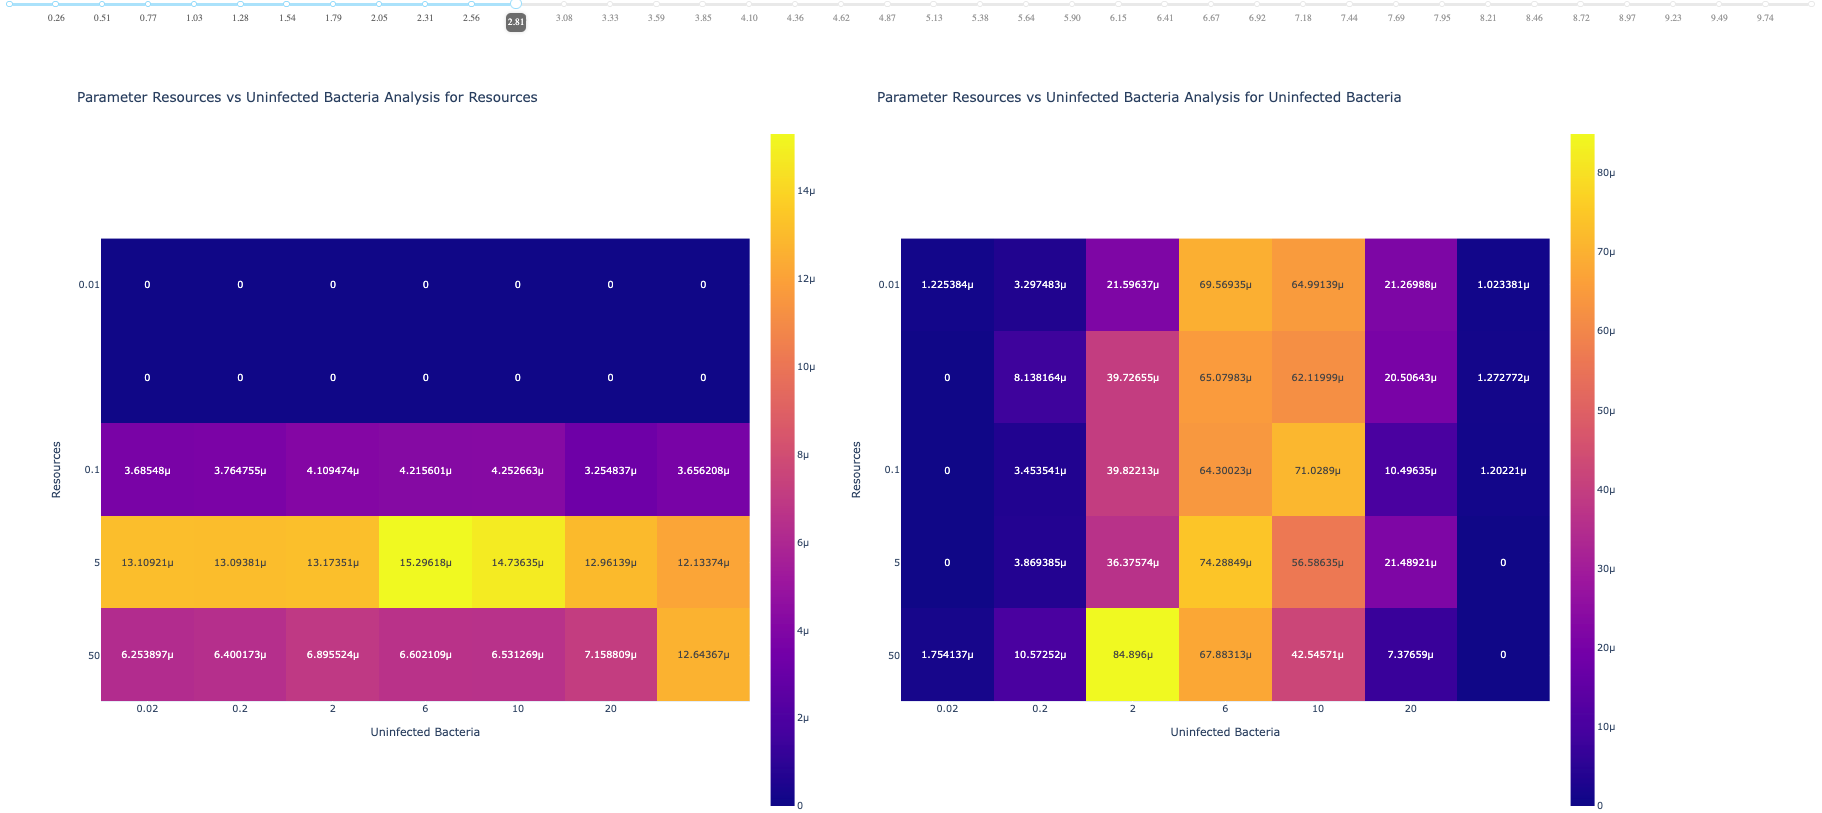
\includegraphics[width=\linewidth]{Screenshots/AdvancedVisualization/parameter_analysis_run.png}
        \caption{
            The expected parameter anlaysis output. 
        }
        \label{fig:ss:av:parameter_analysis_run}
    \end{subfigure}
    \caption{Parameter Analysis}
\end{figure}


\paragraph{Initial Value Analysis}
\label{sec:initial_value_analysis}
The initial value analysis (IVA) settings tab as shown in \Cref{fig:ss:av:initial_value_analysis_settings} allows the user to choose a single parameter and vary the value of that parameter, visualizing how a change in parameter value affects the population count of the entities.

\Cref{fig:ss:av:initial_value_analysis_run} shows the plots that the user receives.
For each entity type, there are three plots made.
The left plot shows the population count through time, one line for each parameter value submitted.
The middle plot takes each run and calculates the “percentage from the max value” (default value of $0.95 \rightarrow 95\%$) reached of the peak.
This value is considered the time of peak, and is used to fix some issues that can arise where the population plateaus or only keeps on rising.
The initial value is plotted on the x-axis, with the time at which the max value is reached on the y-axis.
Using the plotted data, a linear or log fit can be created.
In Figure 1 of \citet{mullaExtremeDiversityPhage2024}, they vary the initial bacteria concentration and measure the time until bacterial collapse. 
The initial concentration and corresponding collapse time are plotted on logarithmic x and y axes, with a linear regression fitted to the log-transformed data.
The observed logarithmic decrease suggests that the phage kinetics is adsorption-limited. 
\Cref{fig:created:initial_value_analysis_UB_50_500_a_good_plot_2} replicates this graph. 

Using the IVA tool can be useful for understanding how a change in parameter value affects the time at which the population count reaches a maximum.
The slope, intercept and $R^2$ value is stored and saved in the third plot, a bar chart, with an editable name. 
For every re-run of the IVA, the slope, intercept and $R^2$ value is stored in the bar chart. 
When executed with multiple parameters, this enables comparison of high-level results across various parameters and experimental conditions.

\begin{figure}[h!]
    \centering
    \begin{subfigure}{0.49\linewidth}
        \centering
        \captionsetup{width=1\linewidth}
        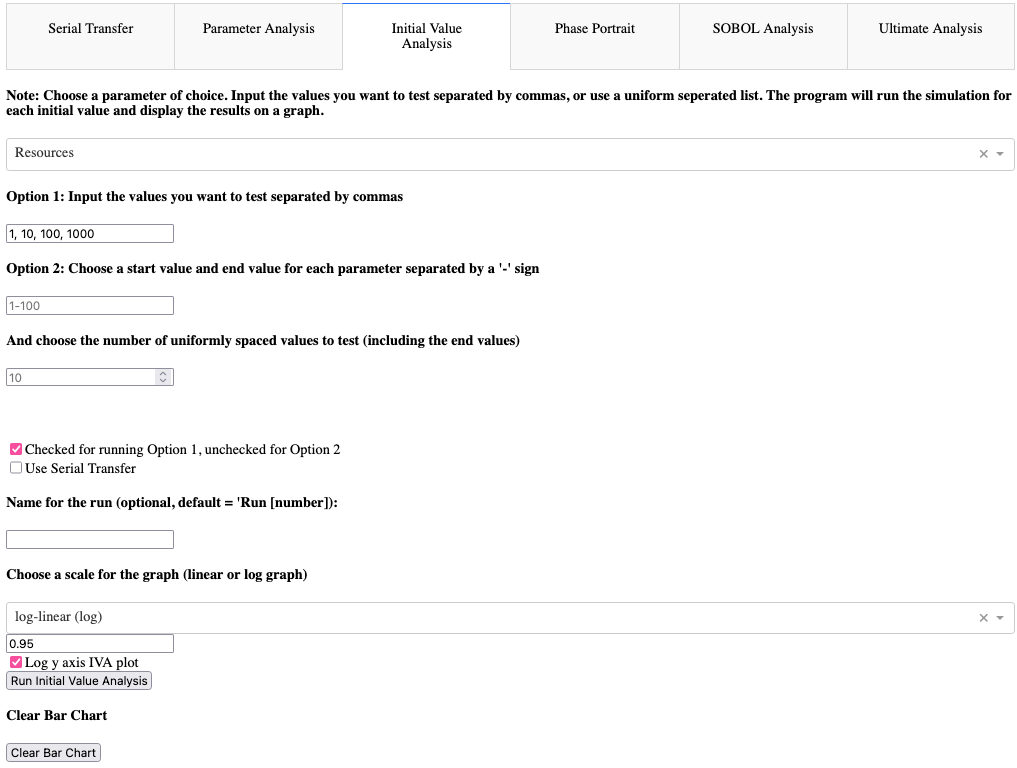
\includegraphics[width=\linewidth]{Screenshots/AdvancedVisualization/initial_value_analysis_settings.png}
        \caption{
            The settings for the IVA tab. 
        }
        \label{fig:ss:av:initial_value_analysis_settings}
        \vspace*{\fill}
    \end{subfigure}
    \hfill
    \begin{subfigure}{0.49\linewidth}
        \centering
        \captionsetup{width=1\linewidth}
        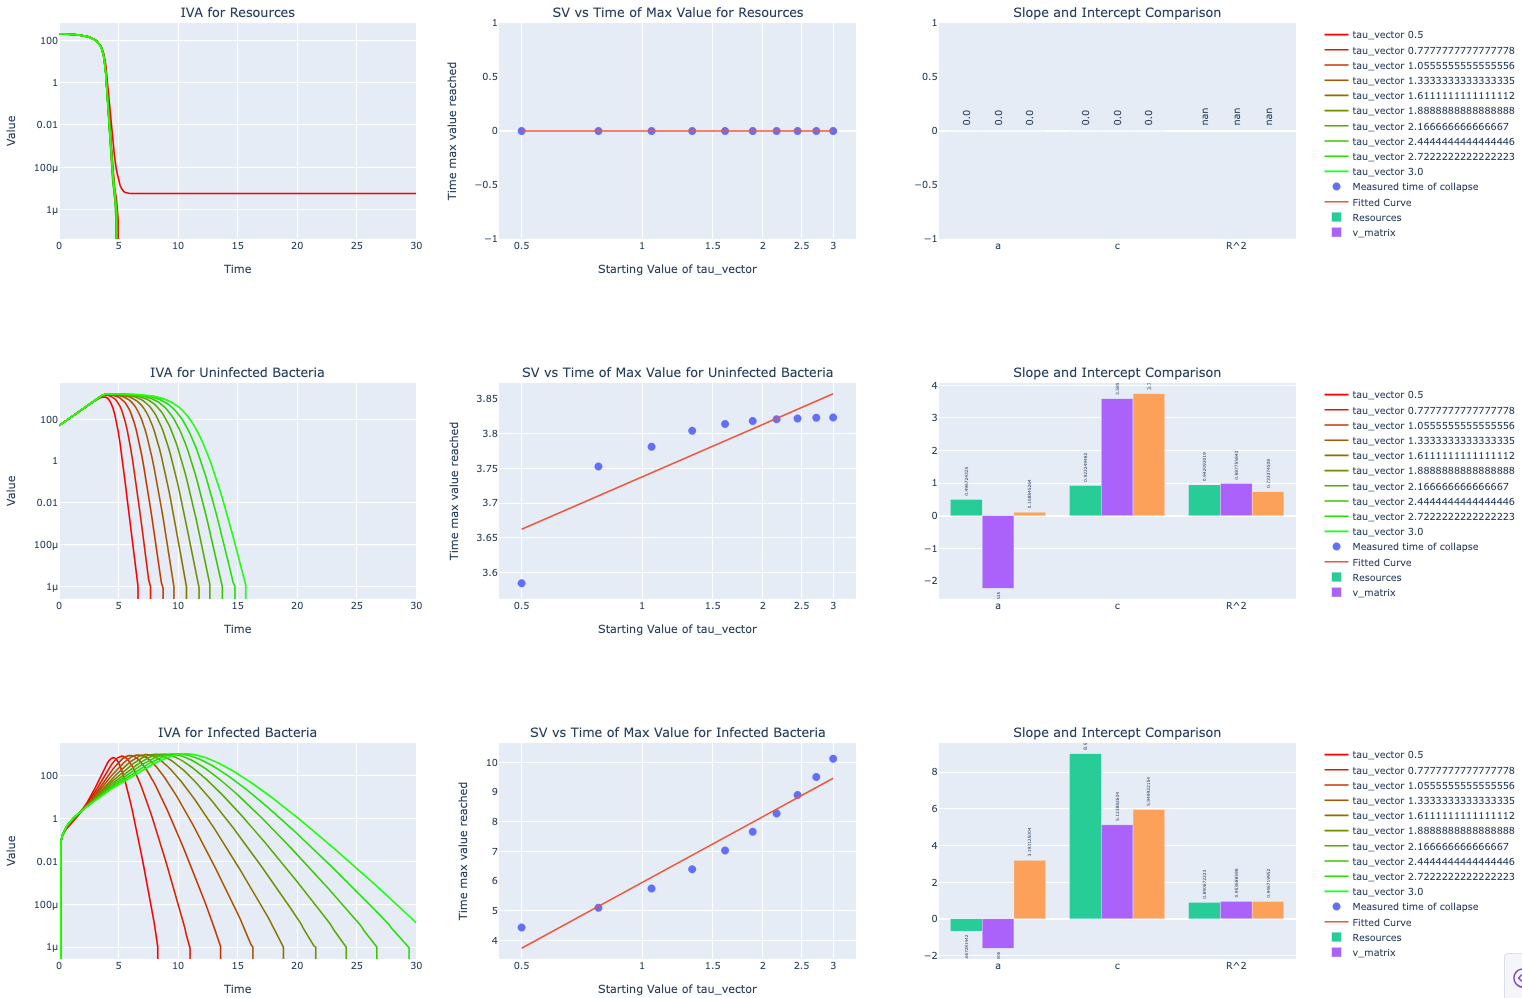
\includegraphics[width=\linewidth]{Screenshots/AdvancedVisualization/initial_value_analysis_run.png}
        \caption{
            An example IVA output. 
        }
        \label{fig:ss:av:initial_value_analysis_run}
        \vspace*{\fill}
    \end{subfigure}
    \caption{The IVA settings and output. }
\end{figure}

\paragraph{Phase Portrait}
\label{sec:phase_portrait}
The phase portrait plot allows the user to analyze how an entity population evolves with respect to the other entity population through time.
Phase portraits indicate how one population increases while the other decreases, and vice versa.
Steady states can be identified and classified as either stable, unstable, or as saddle points. 
It is also possible to visually identify attractor and repeller points by seeing where the population values trend towards. 
By comparing different starting points, it is possible to see if the system is chaotic or not.
The setup for the phase portrait can be seen in \Cref{fig:ss:av:phase_portrait_settings}, and a sample output can be seen in \Cref{fig:ss:av:phase_portrait_run}. 

\begin{figure}[h!]
    \centering
    \begin{subfigure}{0.49\linewidth}
        \centering
        \captionsetup{width=1\linewidth}
        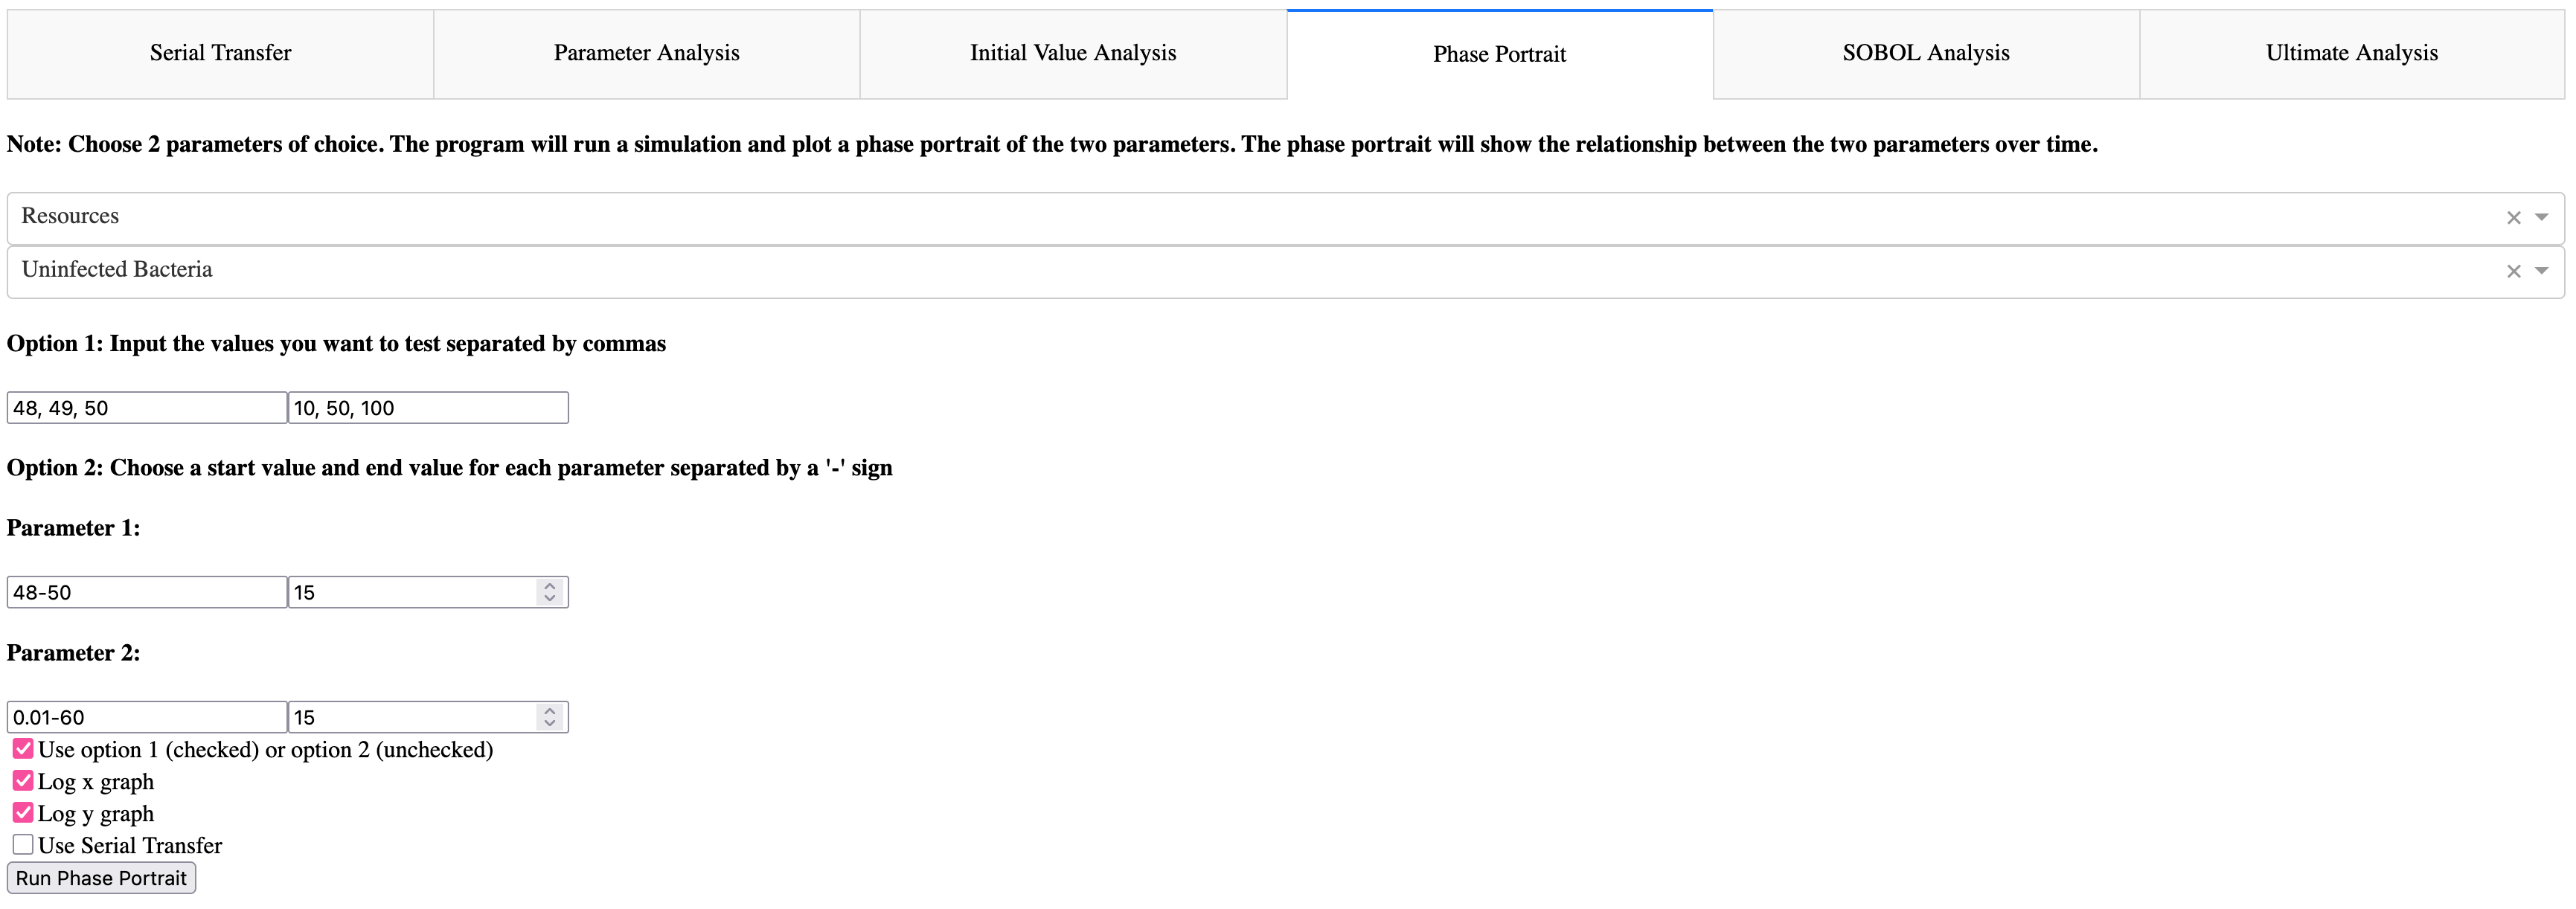
\includegraphics[width=\linewidth]{Screenshots/AdvancedVisualization/phase_portrait_settings.png}
        \caption{
            The user can select two starting values for the IC, but they can't choose vector, matrix, or environment settings due to the plot showing the development of entity populations against other entity populations.
            As typical, the user can select their own values or auto-generate values between two values, as well as use a ST option.
            There is also an option to take the logarithm of the x and/or y-axis. 
        }
        \label{fig:ss:av:phase_portrait_settings}
    \end{subfigure}
    \hfill
    \begin{subfigure}{0.49\linewidth}
        \centering
        \captionsetup{width=1\linewidth}
        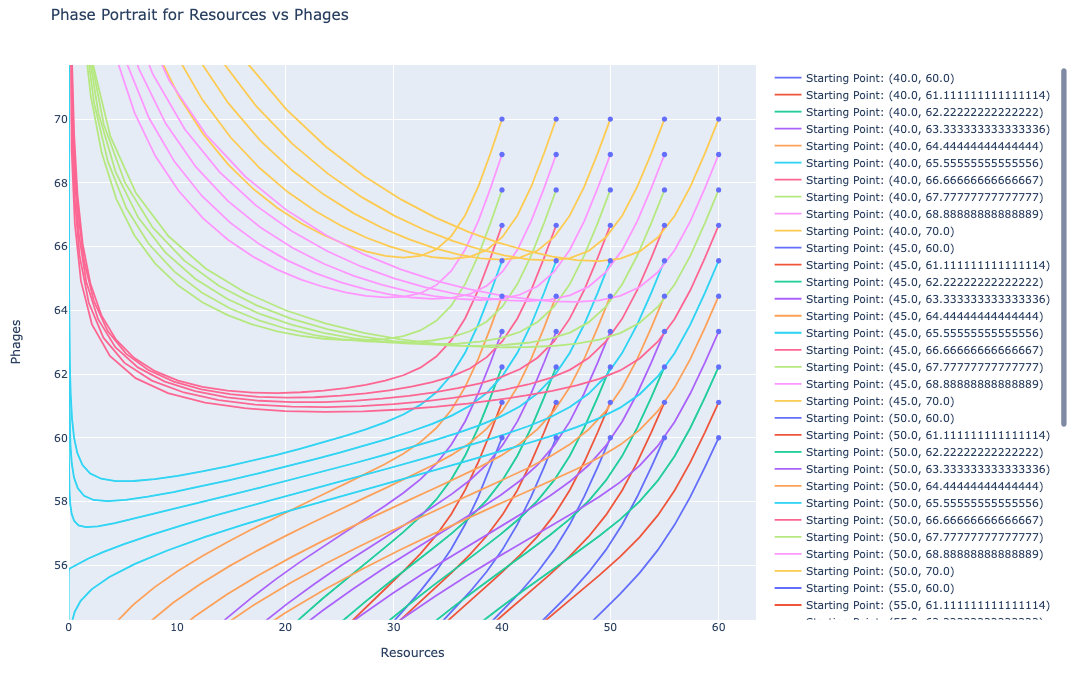
\includegraphics[width=\linewidth]{Screenshots/AdvancedVisualization/phase_portrait_run.png}
        \caption{
            An example phase portrait run. 
        }
        \label{fig:ss:av:phase_portrait_run}
    \end{subfigure}
    \caption{Phase portrait settings and output. }
\end{figure}

\paragraph{SOBOL Sensitivity Analysis}
\label{sec:SOBOL_sensitivity_analysis}
It is important to understand how a change in parameter value affects the change in output of a model. 
Models will have parameters that are more important and have a larger effect on the model output than other parameters. 

SOBOL analysis \cite{sobolGlobalSensitivityIndices2001}, a variance-based sensitivity analysis, is a method that allows a user to quantify how important an input parameter has on a measured aspect of the output by changing the input parameter values of the model and measuring the change in model output.
SOBOL can only measure a single univariate model output, for example the final population value, smallest or largest value reached, the time at which the largest value was reached, or any other univariate output. 
SOBOL quantifies how much variance in the output can be attributed to a specific parameter and can measure the effect of global/total ($ST$), first ($S1$), and second order sensitivity ($S2$). 

First order $Si$, or local sensitivity, is the measurement of the effect that parameter $i$ has on the variance of the output. 
Second order is the measurement of parameter $i$ interacting with parameter $j$, and how the interaction attributes to the output variance. 
Etc for third order and higher. 
Global, also called total sensitivity, is the summation of all interactions. 
If $ST_i \gg S1_i$, then parameter $i$ depends on higher order interactions with other parameters, while when $ST_i \approx S1_i$, then $i$ doesn't interact much with and depend on other parameters.
It should be stated that $ST_i \geq S1_i$ and that $ST_i$ can be greater than 1, while $S1_i \leq 1$. 

When a model is viewed as a black-box model, the model can be seen as a function $Y=f(X)$, where $X$ are the parameter values of $d$ elements, and $Y$ is a univariate model output.
$X$ is assumed to be independently and uniformly distributed within a hypercube $X_i \in [0, 1]$ for $i=1, \dots d$.
The first order sensitivity measures the output variance of the main affect of parameter $X_i$.
Measuring the effect of varying $X_i$ averaged over other input parameters, and standardized to provide a fractional contribution to the overall output variance.
The first order sensitivity is described as
\[
    S1_i = \frac{V_i}{\textit{Var}(Y)}
\] where $V_i = \textit{Var}_{X_i}(\mathbb{E}_{X_{\sim i}}[Y|X_i])$ and where $X_{\sim i}$ represents all the parameters that are not $X_i$.
All parameters are summarized in \Cref{tab:appendixA:parameter_table_SOBOL}

The second order index measures the impact of input $X_i$ interacting with $X_j$. For many inputs, this becomes unwieldy to analyze.
The global sensitivity is used to analyze the global sensitivity without evaluating $2^d-1$ indices, and measures the contribution to the output variance of $X_i$, including all variance due to $X_i$'s interaction with other variables.
\[
    S1_i = \frac{\mathbb{E}_{X_{\sim i}}[\textit{Var}_{X_i}(Y|X_{\sim i}))}{\textit{Var}(Y)} = 1 - \frac{\textit{Var}_{X_i}(\mathbb{E}_{X_i}[Y|X_{\sim i}])}{\textit{Var}(Y)}
\]

SOBOL accepts a list of parameter names and a list of range of values to sample from, which the user can input in the SOBOL settings tab, \Cref{fig:ss:av:SOBOL_analysis_settings}. 
If no values are added, the parameter is not included in the simulation and the default value is instead used. 
The user then needs to select the number of samples to run, using the formula $2^x$, where $x$ is the number they input, and $2^x$ is the number of samples that SOBOL will create and run.
The larger $x$ is, the more accurate the SOBOL analysis results will be, but the more simulations would need to be run.
If 2nd order is not chosen, the model is run $N(D+2)$ times.
If the user wants to analyze the second order interactions, then the model will run the system $N(2D+2)$ times with the randomly sampled input values, where $N$ is a multiple of 2, and $D$ is the number of parameters being tested.
Due to the randomness of the sampling method, the user can, but does not need to, submit a seed value. 

The global and first sensitivity are shown next to one another, and each sub-row within a plot represents each entity type. 
The proportion of the global and local sensitivity can be seen for each entity type and each parameter.

Upon completion of a SOBOL analysis, the original simulation data is saved to the disk as a \textit{.pickle} file so that the user can reuse the data and run their own SOBOL analyses. 

\begin{figure}[h!]
    \centering
    \begin{subfigure}{0.49\linewidth}
        \centering
        \captionsetup{width=1\linewidth}
        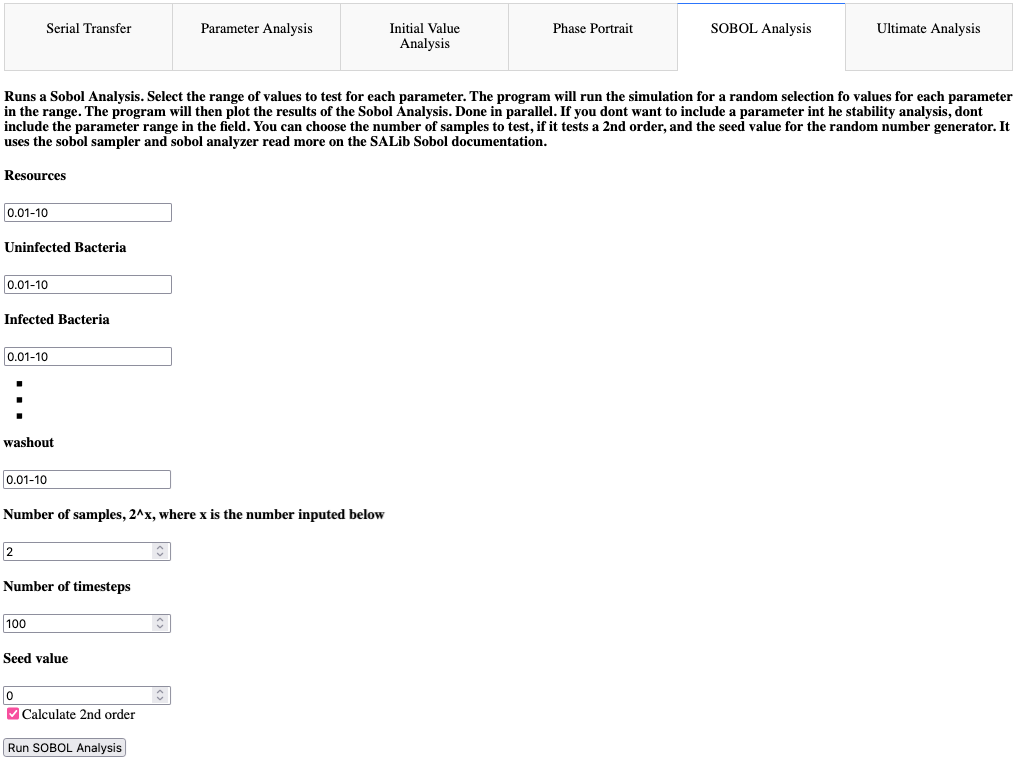
\includegraphics[width=\linewidth]{Screenshots/AdvancedVisualization/SOBOL_analysis_settings.png}
        \caption{
            The SOBOL settings tab. 
        }
        \label{fig:ss:av:SOBOL_analysis_settings}
    \end{subfigure}
    \hfill
    \begin{subfigure}{0.49\linewidth}
        \centering
        \captionsetup{width=1\linewidth}
        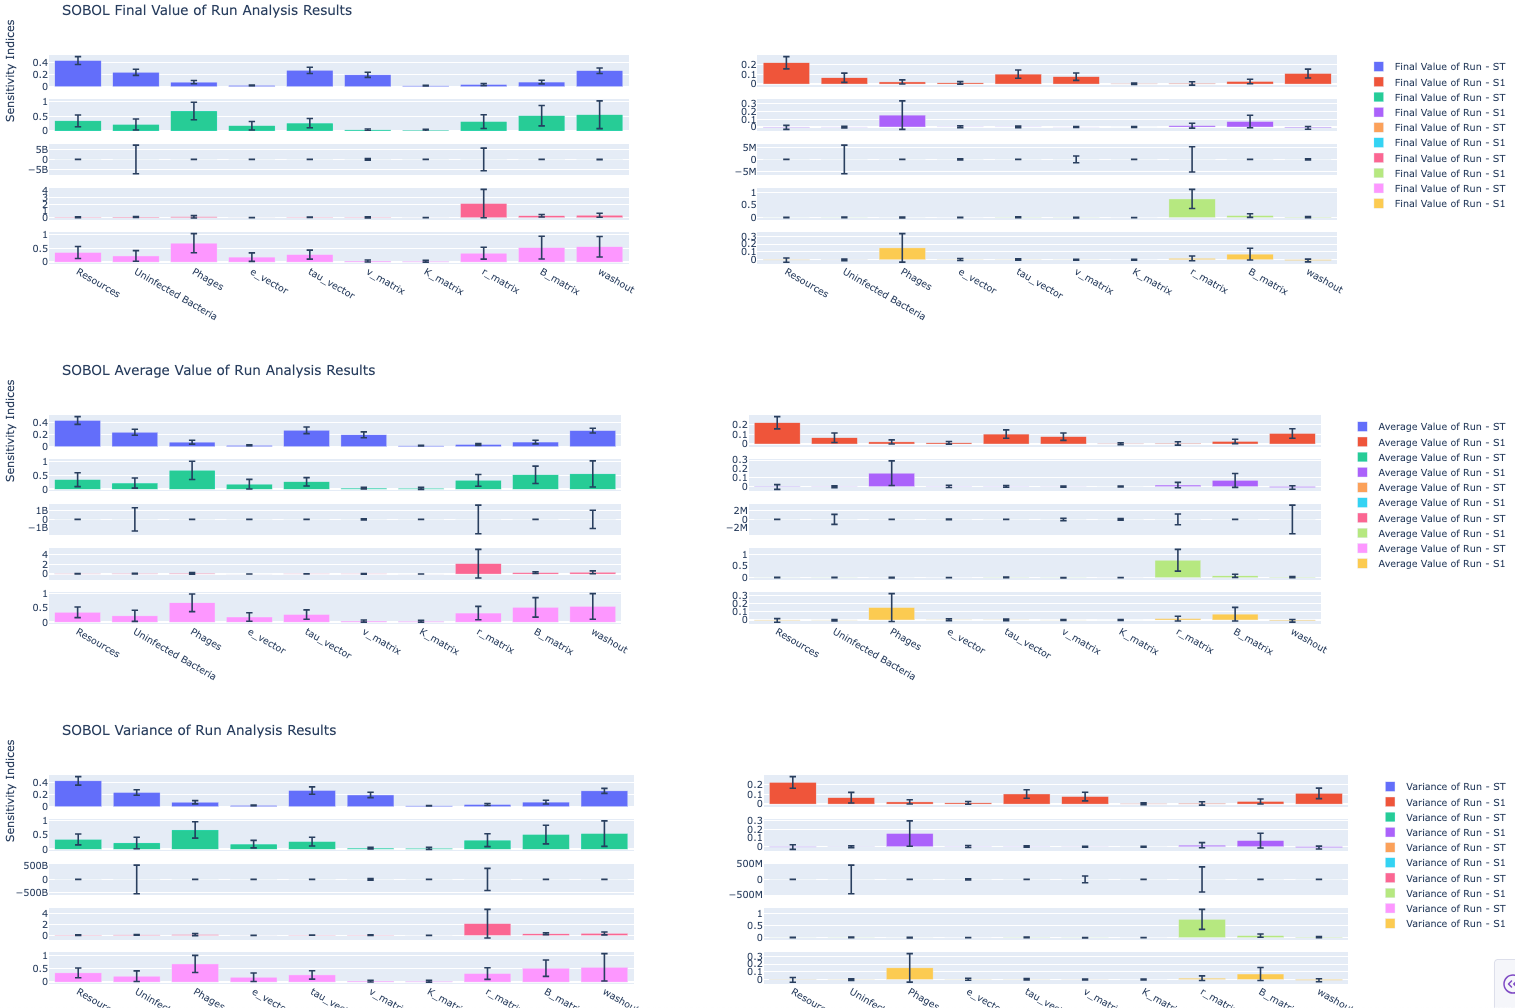
\includegraphics[width=\linewidth]{Screenshots/AdvancedVisualization/SOBOL_analysis_run.png}
        \caption{
            The output that can be expected from SOBOL. 
        }
        \label{fig:ss:av:SOBOL_analysis_run}
    \end{subfigure}
    \caption{SOBOL variance analysis settings and output. }
\end{figure}

\paragraph{Ultimate Analysis}
\label{sec:ultimate_analysis}
Making a dashboard that can be used for different inputs is hard to make. Predicting the type of plots that a user might be interested in, and the type of behavior the user wants to analyze is impossible to predict. 
The Ultimate Analysis section does not produce any visualizations or analysis, but instead allows for the user to define which ICs and parameter values they want to run a simulation on.
The solver will iterate over every single parameter input possibility and save the results in a \textit{.parquet} file.
Similarly settings in the other sections, the user can specify a start and end value, along with the number of values to generate evenly spaced within that range, including both the start and end values (\Cref{fig:ss:av:ultimate_analysis_settings}).
\newline
Using Dask and the saved \textit{.parquet} file, the user can query for specific runs, for example runs where a parameter value was greater than 0.05, and use the simulation data to create their own plots.
\begin{figure}
    \centering
    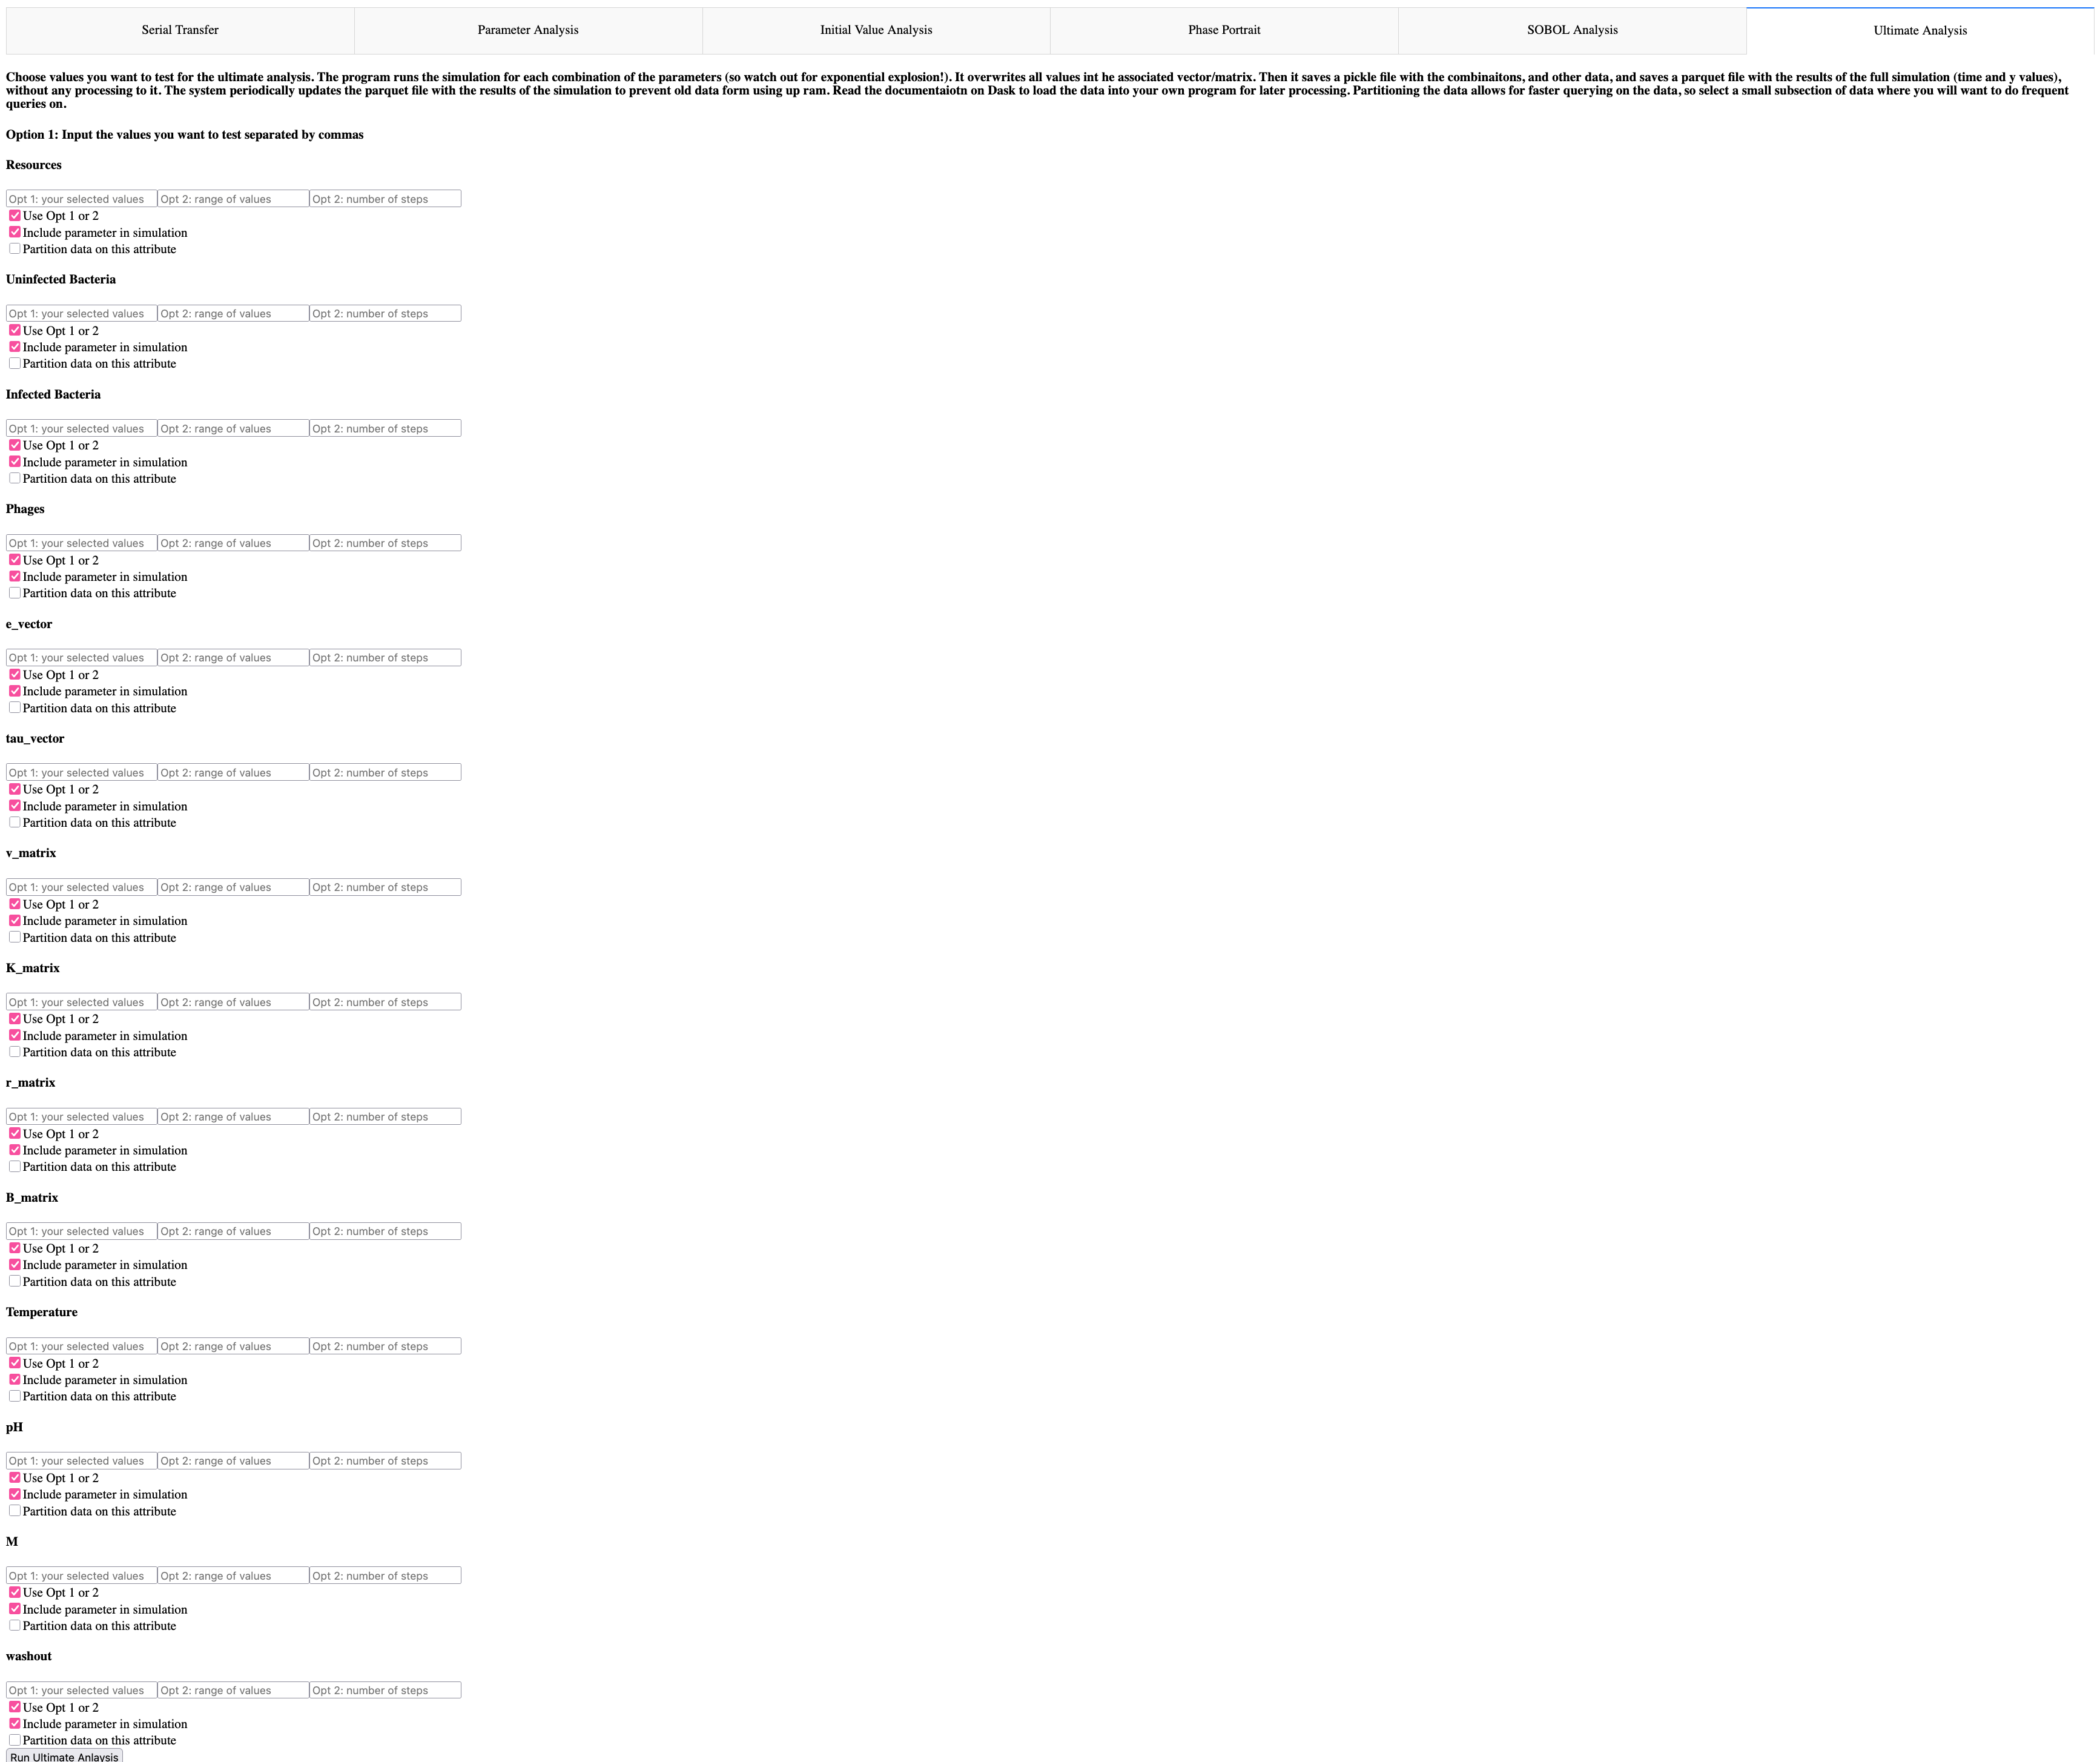
\includegraphics[width=1\linewidth]{Screenshots/AdvancedVisualization/ultimate_analysis_settings.png}
    \caption{
        The ultimate analysis setup tab. 
    }
    \label{fig:ss:av:ultimate_analysis_settings}
\end{figure}

\subsection{Custom Visualizations and Analyses} 
\label{sec:custom_visualizations_and_framework}
The final part, an optional step, allows the user to define a number of parameters they want to simulate and download the simulation results. 
The user can use this data to create their own custom visualizations without having to rerun the simulations, especially if there are many simulations. 
The data can be further processed and visualized as the user wishes. 

As the dashboard can not create a graph for every situation, or be easily adapted to analyze every situation, \Cref{sec:ultimate_analysis} can be used to run and download the simulation data to the disk to later create your own custom visualizations. 

\section{Software Used and Packages}
The program was created exclusively in Python \cite{Python}, and makes extensive usages of various packages, ranging from the standard scientific packages such as NumPy \cite{NumPy} and SciPy to more niche packages such as pickle and SALib \cite{iwanagaSALib20Advancing2022, hermanSALibOpensourcePython2017}.

The graphical tool uses Tkinter acting as the front end, handling the user inputs, while NetworkX \cite{hagbergExploringNetworkStructure2008} stores the graph and contains the attribute data of the edges and nodes. 
The GUI tool also uses Matplotlib \cite{Matplotlib} to create the figure of the graph to display to the user in the GUI tool.

The simulation framework, the backend of the modelling, makes extensive usage of SciPy's \textit{solve\_ivp()} to create the ODE data. 
It also makes light usage of NetworkX to load the graph and parameter values, as it initially takes a graph as an input. 
NumPy is used to set the parameters up at program startup. 

The visualization part makes heavy usage of Dash and Plotly. 
Dash acts as the server and is used for displaying the HTML aspect of the frontend and dealing with any input and output. 
Upon choosing parameter values and clicking on “submit“, Dash registers the activity and calls the function registered to the button, sending data such as parameter values and options like “log x-axis” form the frontend to the backend server. 
In the backend, the various inputs are handled, like changing the input string \textit{“0.05, 0.1, 0.15, 0.2”} into an iterable list \textit{[0.05, 0.1, 0.15, 0.2]} that the simulation framework can iterate over to vary the parameter value. 

If there are many simulations to run through, in the case of \Cref{sec:ultimate_analysis}, an intermediate call to a parallel computing library Joblib is called. 
Joblib parallelizes the computations on multiple CPUs to speed up computing time. 

Ultimate analysis uses Pandas to write the data to a \textit{.parquet} file. 
Pandas parquet offers efficient data compression, efficient memory usage and when combined with Dask, efficient querying functionalities in a Dataframe format that many data scientists would be familiar with. 

SOBOL uses the SALib library to sample and analyze the parameter input. 
Both ultimate analysis and SOBOL save a \textit{.pickle} file containing a dictionary with the parameter values tested, setting values, and other important information regarding the simulation. 

\Cref{sec:initial_value_analysis} uses SciPy's \textit{curve\_fit()} function to curve fit the points in the middle plot (\Cref{fig:ss:av:initial_value_analysis_run}). 

Other packages that are used include collections, copy, warnings, itertools, os, datetime, json, gc, and time. 

